% !TeX program = xelatex
% !TeX encoding = UTF-8
% Spedizione P04 · Un geyser: associazione e previsione
% Presentazione della spedizione P04 nella serie planetaria di GeoStat Lab.
% Compilazione: xelatex -interaction=nonstopmode P04_Geyser.tex (due passaggi)
% 31 slide. Diagrammi TikZ, figure vettoriali da R/P04_figure.R, codice R, dati ed esperimenti inclusi.
\RequirePackage{fix-cm}
\documentclass[12pt,aspectratio=1610]{beamer}
\geometry{paperwidth=20cm,paperheight=12.5cm}
\usepackage[italian,provide=*]{babel}
\usepackage{fontspec,adjustbox,tabularx}
\IfFontExistsTF{NimbusSans-Regular.otf}{
\setsansfont{NimbusSans-Regular.otf}[BoldFont=NimbusSans-Bold.otf,ItalicFont=NimbusSans-Italic.otf,BoldItalicFont=NimbusSans-BoldItalic.otf]
\setmainfont{NimbusSans-Regular.otf}[BoldFont=NimbusSans-Bold.otf,ItalicFont=NimbusSans-Italic.otf,BoldItalicFont=NimbusSans-BoldItalic.otf]
}{
\setsansfont{TeX Gyre Heros}
\setmainfont{TeX Gyre Heros}
}
\IfFontExistsTF{DejaVu Sans Mono}{
\setmonofont{DejaVu Sans Mono}[Scale=.88]
}{\setmonofont{Latin Modern Mono}[Scale=.88]}
\usefonttheme{professionalfonts}
\usepackage{amsmath,amssymb,booktabs,array,graphicx,tikz,bookmark}
\usetikzlibrary{calc,positioning,arrows.meta}
\graphicspath{{Figure/}}
\definecolor{Paper}{HTML}{F8F6F1}
\definecolor{Ink}{HTML}{253344}
\definecolor{Navy}{HTML}{15283E}
\definecolor{Quantum}{HTML}{5146A5}
\definecolor{Classical}{HTML}{087C74}
\definecolor{Muted}{HTML}{657180}
\definecolor{Rule}{HTML}{D6DAD9}
\definecolor{Night}{HTML}{112236}
\definecolor{Lilac}{HTML}{ABB5FF}
\definecolor{Mint}{HTML}{72D8C8}
\setbeamercolor{background canvas}{bg=Paper}
\setbeamercolor{normal text}{fg=Ink}
\setbeamertemplate{navigation symbols}{}
\setbeamertemplate{headline}{}
\setbeamertemplate{footline}{}
\setbeamersize{text margin left=0pt,text margin right=0pt}
\hypersetup{colorlinks=true,linkcolor=Classical,urlcolor=Classical,pdfpagemode=UseOutlines,pdfstartview=Fit,
 pdftitle={Spedizione P04 · Un geyser: associazione e previsione},pdfauthor={GeoStat Lab · materiali di Marzio De Corato},
 pdfsubject={GeoStat Lab · P04}}
\bookmarksetup{open,openlevel=0,depth=2}
\newsavebox{\BodyBox}
\newsavebox{\SideBox}
\newsavebox{\RecallBox}
\newsavebox{\TitleBox}
\newcommand{\MeasureBox}[2]{\typeout{REVIEWBOX:#1:\the\wd#2:\the\ht#2:\the\dp#2}}

% Revisione completa: diagrammi TikZ, formalismo e box R.
\usepackage[most]{tcolorbox}
\usepackage{listings}
\usetikzlibrary{fit,backgrounds,matrix,decorations.pathreplacing}
\definecolor{GeoA}{HTML}{1D7890}
\definecolor{GeoB}{HTML}{C57E42}
\definecolor{GeoC}{HTML}{7363AA}
\definecolor{GeoTint}{HTML}{F0F4F3}
\lstdefinestyle{GeoR}{language=R,basicstyle=\ttfamily\fontsize{9.2}{12.2}\selectfont,
 keywordstyle=\color{Quantum}\bfseries,commentstyle=\color{Classical},stringstyle=\color{GeoB},
 numbers=left,numberstyle=\tiny\color{Muted},numbersep=4pt,showstringspaces=false,
 columns=fullflexible,keepspaces=true,breaklines=true,xleftmargin=1.15em,
 frame=none,aboveskip=0pt,belowskip=0pt,tabsize=2}
\newsavebox{\PilotLeftBox}
\newsavebox{\PilotRightBox}
\newcommand{\PLabel}[1]{\par{\color{Classical}\bfseries\fontsize{9}{11}\selectfont\MakeUppercase{#1}}\par\vspace{1.8mm}}
\newcommand{\PBody}[1]{\par{\fontsize{11.3}{14.8}\selectfont #1\par}}
\newcommand{\PSmall}[1]{\par{\fontsize{9.8}{13.1}\selectfont #1\par}}
\newcommand{\PCode}[2]{%
\begin{tcolorbox}[enhanced,arc=1.8mm,boxrule=.65pt,
  colback=white,colframe=Classical!75!Navy,colbacktitle=Navy,
  coltitle=white,fonttitle=\bfseries\fontsize{9.6}{12}\selectfont,
  title={#1},left=1.7mm,right=1.3mm,top=1.5mm,bottom=1.3mm,
  before skip=1mm,after skip=1mm]
\lstinputlisting[style=GeoR]{Codice/#2}
\end{tcolorbox}}
\newcommand{\PInfo}[1]{%
\begin{tcolorbox}[enhanced,arc=1.6mm,boxrule=.55pt,colback=GeoTint,
 colframe=Rule!80!Classical,left=2.3mm,right=2.3mm,top=2mm,bottom=2mm,
 before skip=1mm,after skip=1mm]
\PSmall{#1}\end{tcolorbox}}
\tikzset{
 pFlow/.style={draw=Classical!45,fill=white,rounded corners=2mm,
  line width=.7pt,align=center,minimum height=1.1cm,font=\sffamily\fontsize{10}{12}\selectfont},
 pEdge/.style={-{Latex[length=2.3mm]},draw=Classical,line width=.95pt},
 pGroup/.style={draw=Rule,fill=white,rounded corners=2mm,line width=.65pt},
 pDotA/.style={circle,fill=GeoA,inner sep=1.25pt},
 pDotB/.style={circle,fill=GeoB,inner sep=1.25pt},
 pDotC/.style={circle,fill=GeoC,inner sep=1.25pt}
}
\newcommand{\PilotChrome}[4]{%
  \node[anchor=north west,inner sep=0,text width=17.7cm] at ([xshift=.95cm,yshift=-.55cm]current page.north west) {\color{Navy}\bfseries\fontsize{20.6}{24.5}\selectfont #1};
  \node[anchor=north east,inner sep=0] at ([xshift=19.05cm,yshift=-.14cm]current page.north west) {\color{Classical}\fontsize{8}{10}\selectfont\hyperlink{slide2}{#2}};
  \draw[Classical,line width=1.2pt] ([xshift=.95cm,yshift=-1.7cm]current page.north west)--([xshift=2.35cm,yshift=-1.7cm]current page.north west);
  \draw[Rule,line width=.65pt] ([xshift=.95cm,yshift=-10.36cm]current page.north west)--([xshift=19.05cm,yshift=-10.36cm]current page.north west);
  \node[anchor=north west,inner sep=0] at ([xshift=.96cm,yshift=-10.55cm]current page.north west) {\color{Classical}\bfseries\fontsize{9.1}{12}\selectfont DA RICORDARE};
  \node[anchor=north west,inner sep=0,text width=14.3cm] at ([xshift=4.2cm,yshift=-10.53cm]current page.north west) {\color{Ink}\fontsize{10.3}{13.8}\selectfont #4};
  \draw[Rule,line width=.35pt] ([xshift=.95cm,yshift=-11.92cm]current page.north west)--([xshift=19.05cm,yshift=-11.92cm]current page.north west);
  \node[anchor=north west,inner sep=0] at ([xshift=.95cm,yshift=-12.06cm]current page.north west) {\color{Muted}\fontsize{7.7}{9.2}\selectfont Spedizione P04 · Un geyser: associazione e previsione};
  \node[anchor=north east,inner sep=0] at ([xshift=19.05cm,yshift=-12.06cm]current page.north west) {\color{Muted}\fontsize{7.7}{9.2}\selectfont #3/31};
}


% Stili comuni per i diagrammi scientifici della revisione completa.
\tikzset{
 pAxis/.style={-{Latex[length=2mm]},draw=Muted,line width=.65pt},
 pNote/.style={font=\sffamily\fontsize{9}{11.5}\selectfont,text=Muted,align=center},
 pLabel/.style={font=\sffamily\fontsize{10}{12.5}\selectfont,text=Ink,align=center}
}
\newsavebox{\FullWideBox}
\setlength{\emergencystretch}{1em}




\newcommand{\PLab}[2]{\par{\color{Classical}\bfseries\fontsize{9}{11}\selectfont
\href{#1}{\MakeUppercase{#2}}}\par\vspace{1.8mm}}

\definecolor{Measure}{HTML}{A05B10}\definecolor{Rose}{HTML}{9B4564}\definecolor{Wash}{HTML}{EAE7F6}\definecolor{Gold}{HTML}{EEC184}
\tikzset{arr/.style={-{Stealth[length=2mm]},line width=.8pt,draw=Classical}}
\newcommand{\Colonna}[2]{\begin{adjustbox}{max totalsize={#1}{7.95cm},valign=t}\begin{minipage}[t]{#1}\raggedright\fontsize{11.3}{14.8}\selectfont #2\end{minipage}\end{adjustbox}}
\begin{document}

\begin{frame}[plain]\hypertarget{slide1}{}\bookmark[level=0,page=1]{Spedizione P04}
\begin{tikzpicture}[remember picture,overlay]
\fill[Night](current page.south west) rectangle(current page.north east);
\IfFileExists{Scena/copertina.jpg}{\node[inner sep=0] at(current page.center){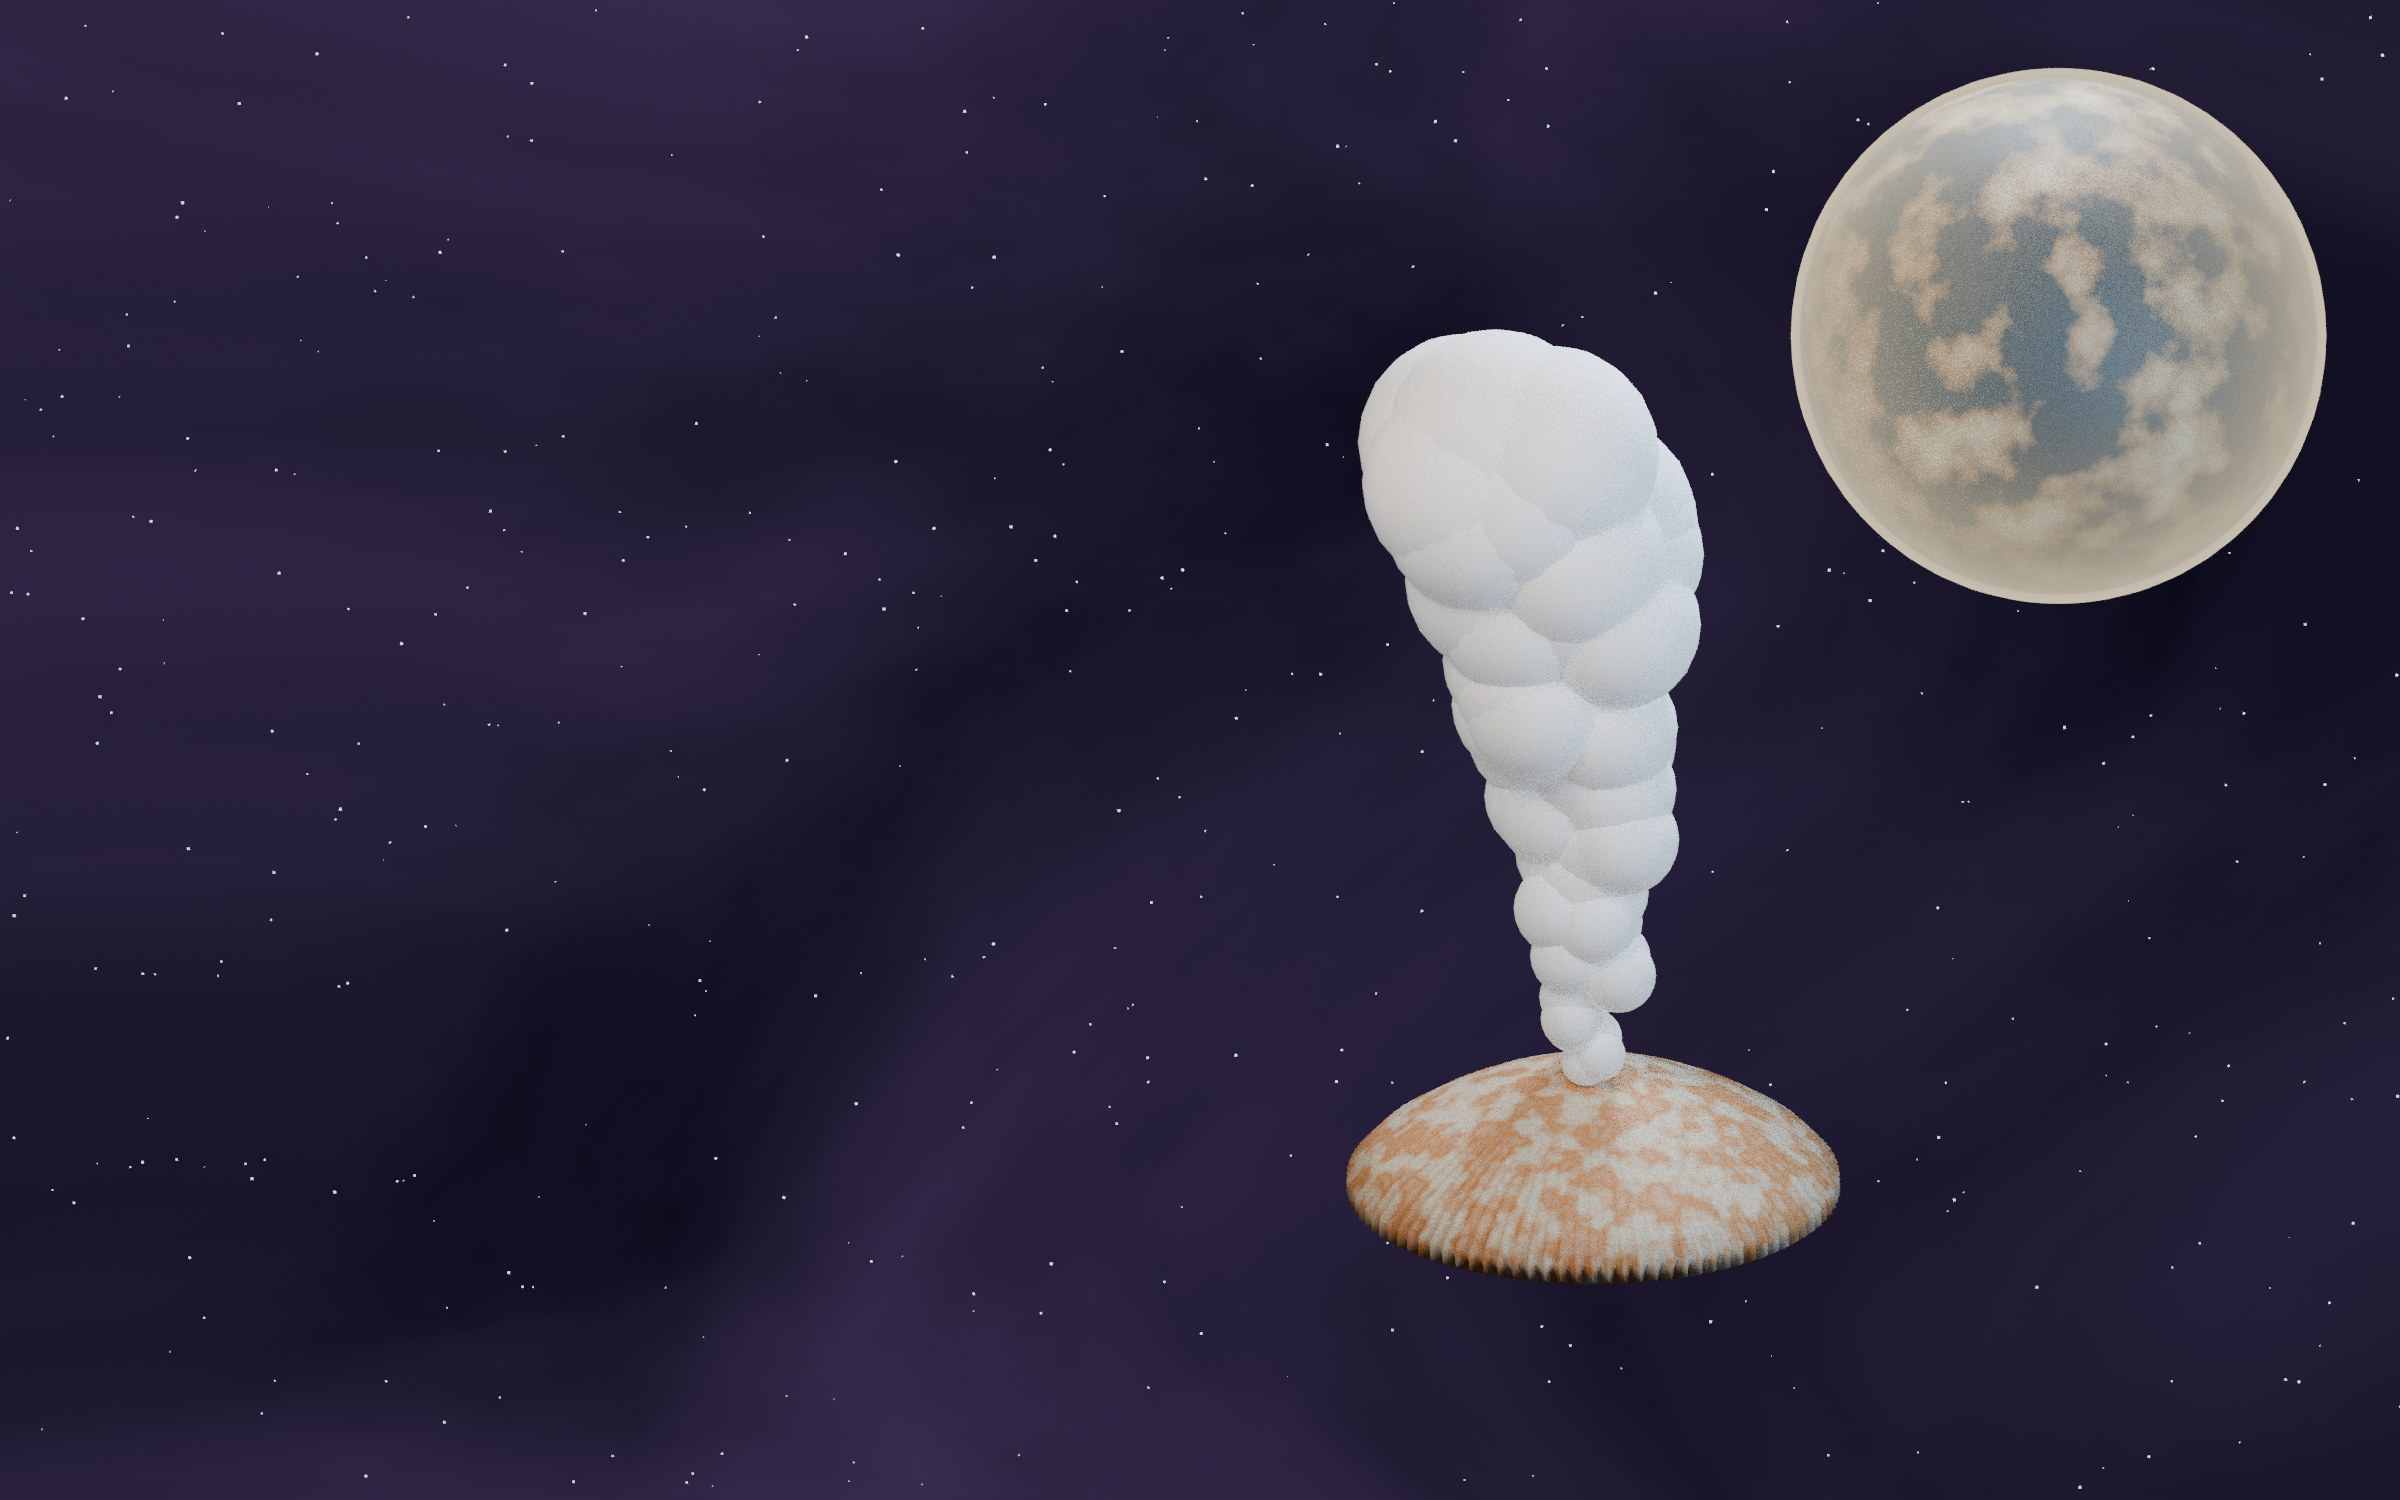
\includegraphics[width=20cm,height=12.5cm]{Scena/copertina.jpg}};}{}
\node[anchor=north west,inner sep=0] at([xshift=1.05cm,yshift=-1.10cm]current page.north west){\color{Mint}\bfseries\fontsize{23}{28}\selectfont SPEDIZIONE P04};
\node[anchor=north west,inner sep=0] at([xshift=1.07cm,yshift=-2.16cm]current page.north west){\color{white}\fontsize{9}{12}\selectfont MACROPROGETTO P04 · SCIENZE DELLA TERRA};
\draw[Mint,line width=1.5pt]([xshift=1.07cm,yshift=-2.78cm]current page.north west)--([xshift=2.6cm,yshift=-2.78cm]current page.north west);
\node[anchor=north west,inner sep=0] at([xshift=1.05cm,yshift=-3.35cm]current page.north west){\begin{minipage}{9.2cm}\raggedright\color{white}\bfseries\fontsize{28.5}{34.5}\selectfont Un geyser:\\associazione\\e previsione\end{minipage}};
\node[anchor=north west,inner sep=0] at([xshift=1.07cm,yshift=-7.88cm]current page.north west){\begin{minipage}{8.9cm}\raggedright\color{Lilac}\fontsize{12.2}{17}\selectfont 272 eruzioni di Old Faithful\end{minipage}};
\node[anchor=north west,inner sep=0] at([xshift=1.07cm,yshift=-8.70cm]current page.north west){\begin{minipage}{8.9cm}\raggedright\color{white!75}\fontsize{10.3}{14.5}\selectfont Durata dell’eruzione, intervalli e valutazione su eventi separati\end{minipage}};
\node[anchor=north west,inner sep=0] at([xshift=1.07cm,yshift=-10.52cm]current page.north west){\color{white}\fontsize{10.5}{14}\selectfont GeoStat Lab · corso di Marzio De Corato};
\node[anchor=north west,inner sep=0] at([xshift=1.07cm,yshift=-11.17cm]current page.north west){\color{Mint}\fontsize{8.8}{11}\selectfont\href{https://creativecommons.org/licenses/by-nc-sa/4.0/}{Impaginazione da Tessera · CC BY-NC-SA 4.0}};
\end{tikzpicture}\end{frame}

\begin{frame}[plain]\hypertarget{slide2}{}
\bookmark[level=1,page=2]{Indice della presentazione}
\begin{tikzpicture}[remember picture,overlay]
\PilotChrome{Indice della presentazione}{PERCORSO}{2}{I titoli dell’indice aprono i capitoli. Il nome del capitolo in alto riporta a questa pagina.}
\node[anchor=north west,inner sep=0] at([xshift=.96cm,yshift=-2.12cm]current page.north west){\Colonna{9.40cm}{\PLabel{Capitoli}
{\fontsize{10.7}{13.5}\selectfont\hyperlink{slide4}{Fonte, bersaglio e separazione dei dati\hfill 4}\par}\vspace{.16cm}
{\fontsize{10.7}{13.5}\selectfont\hyperlink{slide8}{Associazione nel campione di adattamento\hfill 8}\par}\vspace{.16cm}
{\fontsize{10.7}{13.5}\selectfont\hyperlink{slide13}{Incertezza della media e di un evento\hfill 13}\par}\vspace{.16cm}
{\fontsize{10.7}{13.5}\selectfont\hyperlink{slide16}{Valutazione su eventi separati\hfill 16}\par}\vspace{.16cm}
{\fontsize{10.7}{13.5}\selectfont\hyperlink{slide21}{Struttura interna e discussione\hfill 21}\par}\vspace{.16cm}
{\fontsize{10.7}{13.5}\selectfont\hyperlink{slide23}{Laboratori della spedizione\hfill 23}\par}\vspace{.16cm}

}};
\node[anchor=north west,inner sep=0] at([xshift=10.85cm,yshift=-2.12cm]current page.north west){\Colonna{8.16cm}{\PLabel{Percorso di lettura}
\PBody{Il percorso fissa bersaglio e separazione dei dati, descrive l’associazione nel campione di adattamento, distingue l’incertezza della media da quella di un nuovo evento e valuta le previsioni sugli eventi separati. I laboratori finali riprendono le tre fasi della spedizione.}
\PInfo{Le pagine Scenario A e Confronto riprendono gli esperimenti nel browser con dati sintetici. I valori di partenza del simulatore differiscono da quelli del caso.}
\href{https://marzione00.github.io/Lab_Geo/\#modulo-P04}{\color{Classical}\bfseries Apri la spedizione P04 su GeoStat Lab}
}};
\end{tikzpicture}\end{frame}

\begin{frame}[plain]\hypertarget{slide3}{}
\bookmark[level=1,page=3]{Quanto migliora la previsione dell’attesa alla successiva eruzione se si conosce la durata di quella appena conclusa?}
\begin{tikzpicture}[remember picture,overlay]
\PilotChrome{{\fontsize{15.3}{19}\selectfont Quanto migliora la previsione dell’attesa alla successiva eruzione se si conosce la durata di quella appena conclusa?}}{IL CASO GUIDA}{3}{La copertina è una scena illustrativa. Durate e attese provengono dal dataset faithful distribuito con R.}
\node[anchor=north west,inner sep=0] at([xshift=.96cm,yshift=-2.12cm]current page.north west){\Colonna{9.40cm}{{\centering\resizebox{0.97\linewidth}{!}{\begin{tikzpicture}[x=1cm,y=1cm,every node/.style={font=\sffamily\fontsize{10}{12}\selectfont,text=Ink}]
\draw[draw=Classical,fill=Classical!8,rounded corners=2mm,line width=.7pt] (0,0.00) rectangle (8.6,-0.78);
\node[circle,anchor=center,fill=Classical,inner sep=0,minimum size=.5cm,text=white,font=\sffamily\bfseries\fontsize{9}{10}\selectfont] at (.48,-0.39) {1};
\node[anchor=west,text width=7.4cm,align=left] at (.95,-0.39) {Fonte, bersaglio e separazione dei dati};
\draw[pEdge] (.48,-0.80)--(.48,-1.02);
\draw[draw=Classical,fill=Classical!8,rounded corners=2mm,line width=.7pt] (0,-1.04) rectangle (8.6,-1.82);
\node[circle,anchor=center,fill=Classical,inner sep=0,minimum size=.5cm,text=white,font=\sffamily\bfseries\fontsize{9}{10}\selectfont] at (.48,-1.43) {2};
\node[anchor=west,text width=7.4cm,align=left] at (.95,-1.43) {Associazione nel campione di adattamento};
\draw[pEdge] (.48,-1.84)--(.48,-2.06);
\draw[draw=Classical,fill=Classical!8,rounded corners=2mm,line width=.7pt] (0,-2.08) rectangle (8.6,-2.86);
\node[circle,anchor=center,fill=Classical,inner sep=0,minimum size=.5cm,text=white,font=\sffamily\bfseries\fontsize{9}{10}\selectfont] at (.48,-2.47) {3};
\node[anchor=west,text width=7.4cm,align=left] at (.95,-2.47) {Incertezza della media e di un evento};
\draw[pEdge] (.48,-2.88)--(.48,-3.10);
\draw[draw=Classical,fill=Classical!8,rounded corners=2mm,line width=.7pt] (0,-3.12) rectangle (8.6,-3.90);
\node[circle,anchor=center,fill=Classical,inner sep=0,minimum size=.5cm,text=white,font=\sffamily\bfseries\fontsize{9}{10}\selectfont] at (.48,-3.51) {4};
\node[anchor=west,text width=7.4cm,align=left] at (.95,-3.51) {Valutazione su eventi separati};
\draw[pEdge] (.48,-3.92)--(.48,-4.14);
\draw[draw=Classical,fill=Classical!8,rounded corners=2mm,line width=.7pt] (0,-4.16) rectangle (8.6,-4.94);
\node[circle,anchor=center,fill=Classical,inner sep=0,minimum size=.5cm,text=white,font=\sffamily\bfseries\fontsize{9}{10}\selectfont] at (.48,-4.55) {5};
\node[anchor=west,text width=7.4cm,align=left] at (.95,-4.55) {Struttura interna e discussione};
\draw[pEdge] (.48,-4.96)--(.48,-5.18);
\draw[draw=GeoB,fill=GeoB!8,rounded corners=2mm,line width=.7pt] (0,-5.20) rectangle (8.6,-5.98);
\node[circle,anchor=center,fill=GeoB,inner sep=0,minimum size=.5cm,text=white,font=\sffamily\bfseries\fontsize{9}{10}\selectfont] at (.48,-5.59) {L};
\node[anchor=west,text width=7.4cm,align=left] at (.95,-5.59) {Laboratori della spedizione};
\end{tikzpicture}
}\par}
\PSmall{Capitoli della spedizione; L indica i laboratori conclusivi.}
}};
\node[anchor=north west,inner sep=0] at([xshift=10.85cm,yshift=-2.12cm]current page.north west){\Colonna{8.16cm}{\PLabel{Il caso}
\PBody{Il dataset faithful di R contiene 272 coppie di durata dell’eruzione e attesa alla successiva, in minuti, per il geyser Old Faithful. Una separazione fissata prima dell’esplorazione destina 190 eventi all’adattamento e 82 alla verifica.}
\PInfo{Seguiremo la retta dalla pendenza media all’intervallo per un nuovo evento, fino all’errore misurato sugli eventi tenuti separati.}
}};
\end{tikzpicture}\end{frame}

\begin{frame}[plain]\hypertarget{slide4}{}
\bookmark[level=0,page=4]{Fonte, bersaglio e separazione dei dati}
\bookmark[level=1,page=4]{Definire il bersaglio prima del modello}
\begin{tikzpicture}[remember picture,overlay]
\PilotChrome{Definire il bersaglio prima del modello}{FONTE, BERSAGLIO E SEPARAZIONE DEI DATI}{4}{Il bersaglio operativo richiede un’origine temporale coerente con l’informazione disponibile.}
\node[anchor=north west,inner sep=0] at([xshift=.96cm,yshift=-2.12cm]current page.north west){\Colonna{9.40cm}{{\centering\resizebox{0.90\linewidth}{!}{\begin{tikzpicture}[x=1cm,y=-.87cm,every node/.style={font=\fontsize{12.2}{15}\selectfont,text=Ink},arr/.style={-{Stealth[length=2mm]},line width=.8pt,draw=Classical}]\path[use as bounding box] (0,0) rectangle (7.45,6.2);
\draw[Rule,line width=.8pt] (0.5,2.3)--(7,2.3);
\draw[draw=Classical,fill=Classical!8,rounded corners=2pt,line width=.7pt] (1,1.7) rectangle (3.2,2.9);
\node[anchor=center,text=Ink,font=\fontsize{12.2}{15}\selectfont,text width=2.7cm,align=center] at (2.1,1.1) {Eruzione};
\draw[Quantum,line width=.8pt] (3.2,3.3)--(3.2,4.2);
\node[anchor=center,text=Ink,font=\fontsize{11.5}{15}\selectfont,text width=3.7cm,align=center] at (3.2,5) {Durata completa disponibile};
\node[anchor=center,text=Ink,font=\fontsize{11.5}{15}\selectfont,text width=2.7cm,align=center] at (6,1.1) {Evento seguente};
\draw[Quantum,line width=.8pt] (6,1.7)--(6,2.9);
\draw[arr,draw=Quantum] (3.5,3.5)--(5.8,3.5);
\node[anchor=center,text=Ink,font=\fontsize{11.5}{15}\selectfont,text width=2.7cm,align=center] at (5.1,4.3) {Tempo residuo};

\end{tikzpicture}}\par}
}};
\node[anchor=north west,inner sep=0] at([xshift=10.85cm,yshift=-2.12cm]current page.north west){\Colonna{8.16cm}{\PBody{Il dataset faithful contiene 272 coppie di durata dell’eruzione e attesa alla successiva, espresse in minuti. Il progetto esamina se la durata migliori la previsione dell’attesa rispetto a una previsione costante. La durata completa è disponibile soltanto al termine dell’eruzione, mentre l’estratto non fornisce date e protocollo dettagliato dell’origine dei tempi. Un’applicazione operativa dovrebbe quindi verificare anche se l’attesa sia misurata dall’inizio o dalla fine dell’evento, traducendo il bersaglio nel tempo residuo effettivamente disponibile al momento della previsione.}
}};
\end{tikzpicture}\end{frame}

\begin{frame}[plain]\hypertarget{slide5}{}
\bookmark[level=1,page=5]{La fonte conserva arrotondamenti e limiti storici}
\begin{tikzpicture}[remember picture,overlay]
\PilotChrome{La fonte conserva arrotondamenti e limiti storici}{FONTE, BERSAGLIO E SEPARAZIONE DEI DATI}{5}{L’uguaglianza di valori arrotondati va distinta dalla duplicazione accidentale di una registrazione.}
\node[anchor=north west,inner sep=0] at([xshift=.96cm,yshift=-2.12cm]current page.north west){\Colonna{9.40cm}{\PBody{La tabella riproduce i valori distribuiti con R e conserva un identificativo di riga, costruito per rendere ripetibile la separazione dei dati. La documentazione segnala arrotondamenti nei tempi, per cui coppie numericamente uguali possono rappresentare eventi distinti. Il controllo confronta i valori con faithful e verifica positività e identificativi, evitando cancellazioni automatiche. L’assenza delle date impedisce di costruire una vera verifica prospettica della stabilità nel tempo e limita l’interpretazione del test a una generalizzazione interna sotto scambiabilità.}
}};
\node[anchor=north west,inner sep=0] at([xshift=10.85cm,yshift=-2.12cm]current page.north west){\Colonna{8.16cm}{\PInfo{Il dataset storico riguarda Old Faithful nello Yellowstone. Le unità in minuti e le convenzioni della fonte devono essere mantenute nel modello. Un risultato ottenuto su questo estratto richiederebbe nuove osservazioni cronologiche e verifiche del protocollo prima di sostenere una prestazione operativa attuale.}
}};
\end{tikzpicture}\end{frame}

\begin{frame}[plain]\hypertarget{slide6}{}
\bookmark[level=1,page=6]{Una separazione condivisa prima dell’esplorazione}
\begin{tikzpicture}[remember picture,overlay]
\PilotChrome{Una separazione condivisa prima dell’esplorazione}{FONTE, BERSAGLIO E SEPARAZIONE DEI DATI}{6}{La separazione riguarda tutte le decisioni che possono utilizzare l’informazione della risposta.}
\node[anchor=north west,inner sep=0] at([xshift=.96cm,yshift=-2.12cm]current page.north west){\Colonna{9.40cm}{{\centering\resizebox{0.90\linewidth}{!}{\begin{tikzpicture}[x=1cm,y=-.87cm,every node/.style={font=\fontsize{12.2}{15}\selectfont,text=Ink},arr/.style={-{Stealth[length=2mm]},line width=.8pt,draw=Classical}]\path[use as bounding box] (0,0) rectangle (7.45,6.2);
\draw[draw=Classical,fill=Classical!8,rounded corners=2pt,line width=.7pt] (0.5,0.6) rectangle (6.9,1.9);
\node[anchor=center,text=Ink,font=\fontsize{12.2}{15}\selectfont,text width=6cm,align=center] at (3.7,1.25) {272 eventi identificati};
\draw[arr,draw=Classical] (2,2.1)--(2,3);
\draw[arr,draw=Quantum] (5.4,2.1)--(5.4,3);
\draw[draw=Classical,fill=Classical!8,rounded corners=2pt,line width=.7pt] (0.4,3.2) rectangle (3.5,4.8);
\node[anchor=center,text=Ink,font=\fontsize{12}{15}\selectfont,text width=2.8cm,align=center] at (1.95,4) {190: adattamento};
\draw[draw=Quantum,fill=Quantum!8,rounded corners=2pt,line width=.7pt] (3.9,3.2) rectangle (7,4.8);
\node[anchor=center,text=Ink,font=\fontsize{12}{15}\selectfont,text width=2.8cm,align=center] at (5.45,4) {82: verifica};
\node[anchor=center,text=Ink,font=\fontsize{11}{15}\selectfont,text width=6.8cm,align=center] at (3.7,5.7) {Piano fisso; nessun evento appartiene a entrambi.};

\end{tikzpicture}}\par}
}};
\node[anchor=north west,inner sep=0] at([xshift=10.85cm,yshift=-2.12cm]current page.north west){\Colonna{8.16cm}{\PBody{Il piano conservato assegna 190 eventi all’insieme di adattamento e 82 a quello di verifica, mantenendo gli identificativi delle righe. L’esplorazione, la stima dei coefficienti e la costruzione della previsione costante utilizzano soltanto i 190 eventi selezionati per l’adattamento. Gli 82 eventi separati vengono impiegati per valutare le procedure già definite. Poiché la divisione è casuale e manca una cronologia, l’esperimento valuta la generalizzazione entro una popolazione di eventi considerata scambiabile, senza simulare necessariamente le condizioni di una previsione futura.}
}};
\end{tikzpicture}\end{frame}

\begin{frame}[plain]\hypertarget{slide7}{}
\bookmark[level=1,page=7]{Identificativi e separazione verificabile}
\begin{tikzpicture}[remember picture,overlay]
\PilotChrome{Identificativi e separazione verificabile}{FONTE, BERSAGLIO E SEPARAZIONE DEI DATI}{7}{Un piano esplicito conserva l’assegnazione degli eventi indipendentemente dall’ordinamento e dal generatore casuale.}
\node[anchor=north west,inner sep=0] at([xshift=.96cm,yshift=-2.12cm]current page.north west){\Colonna{9.40cm}{\PBody{La separazione viene applicata mediante l’identificativo, così che un ordinamento diverso della tabella non cambi l’appartenenza degli eventi. I controlli sul piano completo, eseguiti nello script integrale, verificano unicità e copertura di tutti gli identificativi prima dell’unione. Il frammento controlla poi numerosità e disgiunzione dei due insiemi. La riproduzione della procedura dipende dal piano salvato, mentre un semplice seme casuale condiviso fra linguaggi non garantirebbe la medesima assegnazione delle righe.}
}};
\node[anchor=north west,inner sep=0] at([xshift=10.85cm,yshift=-2.12cm]current page.north west){\Colonna{8.16cm}{\begin{tcolorbox}[enhanced,arc=1.7mm,boxrule=.6pt,colback=white,colframe=Classical!60!Navy,colbacktitle=Navy,coltitle=white,fonttitle=\bfseries\small,title={R · calcolo riproducibile},left=1.7mm,right=1.3mm,top=1.1mm,bottom=1.1mm,before skip=1mm,after skip=1.0mm]\lstinputlisting[style=GeoR,language=R,basicstyle=\ttfamily\fontsize{8.6}{11.4}\selectfont]{Codice/separazione.R}\end{tcolorbox}
\PLabel{Risultato in R}
\begin{tcolorbox}[colback=GeoTint,colframe=Rule,boxrule=.5pt,arc=1.4mm,left=2mm,right=1mm,top=1mm,bottom=1mm]{\fontsize{8.4}{10.9}\selectfont\ttfamily \mbox{train\ \ test\ }\\\mbox{\ \ 190\ \ \ \ 82\ }}\end{tcolorbox}
}};
\end{tikzpicture}\end{frame}

\begin{frame}[plain]\hypertarget{slide8}{}
\bookmark[level=0,page=8]{Associazione nel campione di adattamento}
\bookmark[level=1,page=8]{La relazione mostra due addensamenti}
\begin{tikzpicture}[remember picture,overlay]
\PilotChrome{La relazione mostra due addensamenti}{ASSOCIAZIONE NEL CAMPIONE DI ADATTAMENTO}{8}{La geometria del campione orienta l’interpretazione della pendenza prima della sua verifica inferenziale.}
\node[anchor=north west,inner sep=0] at([xshift=.96cm,yshift=-2.12cm]current page.north west){\Colonna{9.40cm}{{\centering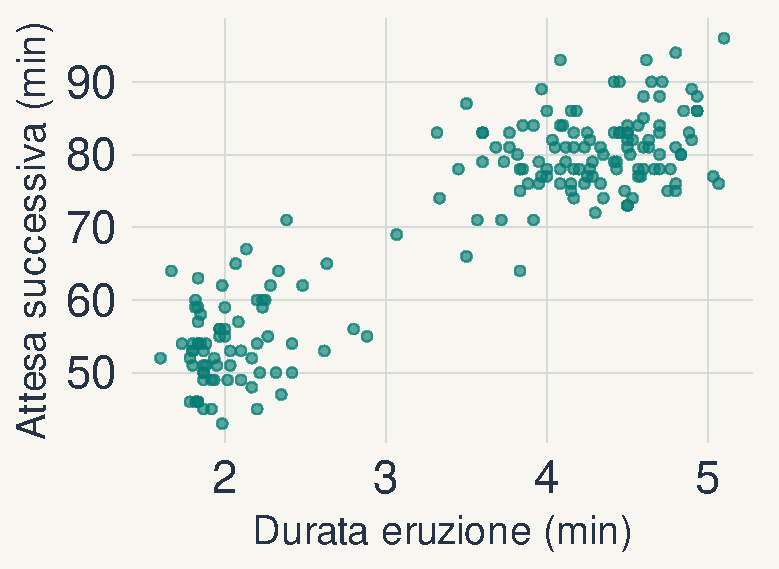
\includegraphics[width=\linewidth,height=6.15cm,keepaspectratio]{Figure/F01.pdf}\par}
\PSmall{Coppie del solo insieme di adattamento. La scala dell’attesa segue la variabile pubblicata nella fonte.}
}};
\node[anchor=north west,inner sep=0] at([xshift=10.85cm,yshift=-2.12cm]current page.north west){\Colonna{8.16cm}{\PBody{Il grafico delle 190 coppie di adattamento mostra una relazione crescente e due addensamenti nella durata e nell’attesa. Questi gruppi visivi suggeriscono una struttura che merita approfondimento, pur senza identificare automaticamente due stati fisici del sistema idrotermale. Una retta globale riassume insieme la separazione fra gli addensamenti e la variazione interna a ciascuno. La sua pendenza dovrà quindi essere interpretata come sintesi dell’associazione nel campione, verificando successivamente quanto differisca dalle pendenze entro intervalli di durata.}
}};
\end{tikzpicture}\end{frame}

\begin{frame}[plain]\hypertarget{slide9}{}
\bookmark[level=1,page=9]{La distribuzione delle durate completa il confronto}
\begin{tikzpicture}[remember picture,overlay]
\PilotChrome{{\fontsize{15.3}{19}\selectfont La distribuzione delle durate completa il confronto}}{ASSOCIAZIONE NEL CAMPIONE DI ADATTAMENTO}{9}{La densità dei predittori determina dove la relazione riceve maggiore sostegno empirico.}
\node[anchor=north west,inner sep=0] at([xshift=.96cm,yshift=-2.12cm]current page.north west){\Colonna{9.40cm}{{\centering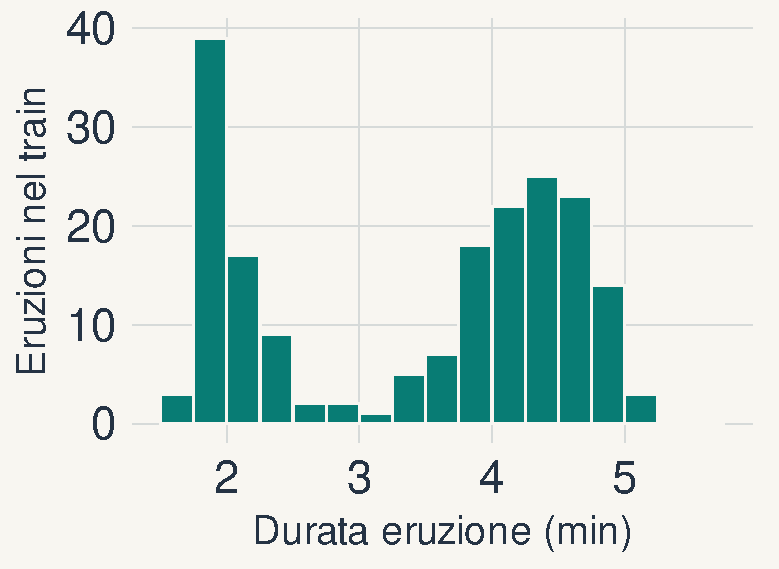
\includegraphics[width=\linewidth,height=6.15cm,keepaspectratio]{Figure/F02.pdf}\par}
\PSmall{Distribuzione delle durate nei 190 eventi di adattamento; intervalli di ampiezza 0,25 minuti.}
}};
\node[anchor=north west,inner sep=0] at([xshift=10.85cm,yshift=-2.12cm]current page.north west){\Colonna{8.16cm}{\PBody{L’istogramma rende esplicita la scarsa densità di eventi nella regione intermedia fra i due addensamenti. La posizione della retta in quella regione dipende dal modello lineare e riceve un sostegno osservativo minore rispetto alle zone più popolate. Gli intervalli delle barre sono fissati in quarti di minuto, mantenendo la scala e gli arrotondamenti della fonte. La lettura congiunta di istogramma e diagramma di dispersione permette di distinguere una relazione osservata diffusamente da una connessione sostenuta soprattutto da gruppi separati.}
}};
\end{tikzpicture}\end{frame}

\begin{frame}[plain]\hypertarget{slide10}{}
\bookmark[level=1,page=10]{La pendenza misura un’associazione media}
\begin{tikzpicture}[remember picture,overlay]
\PilotChrome{La pendenza misura un’associazione media}{ASSOCIAZIONE NEL CAMPIONE DI ADATTAMENTO}{10}{L’interpretazione della pendenza conserva risposta, predittore e dominio del campione utilizzato.}
\node[anchor=north west,inner sep=0] at([xshift=.96cm,yshift=-2.12cm]current page.north west){\Colonna{9.40cm}{\PBody{La regressione collega l’attesa alla durata mediante una retta e un errore di media condizionata nulla. La pendenza stimata è circa 10,898 minuti di attesa per ogni minuto aggiuntivo di durata, mentre il coefficiente di determinazione è circa 0,819. Il coefficiente descrive l’associazione nella specificazione adottata e non identifica l’effetto di un intervento capace di prolungare un’eruzione. L’interpretazione fisica richiede un modello delle condizioni comuni che determinano le due variabili.}
\par\smallskip{\centering\adjustbox{max width=.98\linewidth}{$\displaystyle \begin{gathered}Y_i=\alpha+\beta x_i+\varepsilon_i,\qquad E(\varepsilon_i\mid x_i)=0\\\widehat\beta=\frac{\sum_i(x_i-\overline x)(y_i-\overline y)}{\sum_i(x_i-\overline x)^2}\end{gathered}$}\par\smallskip}
}};
\node[anchor=north west,inner sep=0] at([xshift=10.85cm,yshift=-2.12cm]current page.north west){\Colonna{8.16cm}{\PInfo{$x_i$: durata; $y_i$: attesa osservata, entrambe in minuti. Y indica la risposta casuale; $\alpha$: intercetta; $\beta$: pendenza; $\varepsilon_i$: errore. Le barre sono medie dei 190 eventi di adattamento. La pendenza ha unità min/min: il rapporto descrive due tempi distinti e non una variazione percentuale.}
}};
\end{tikzpicture}\end{frame}

\begin{frame}[plain]\hypertarget{slide11}{}
\bookmark[level=1,page=11]{La covarianza HC3 considera varianze differenti}
\begin{tikzpicture}[remember picture,overlay]
\PilotChrome{La covarianza HC3 considera varianze differenti}{ASSOCIAZIONE NEL CAMPIONE DI ADATTAMENTO}{11}{Una covarianza robusta risponde a una forma dichiarata di deviazione dalle ipotesi classiche.}
\node[anchor=north west,inner sep=0] at([xshift=.96cm,yshift=-2.12cm]current page.north west){\Colonna{9.40cm}{{\centering\resizebox{0.90\linewidth}{!}{\begin{tikzpicture}[x=1cm,y=-.87cm,every node/.style={font=\fontsize{12.2}{15}\selectfont,text=Ink},arr/.style={-{Stealth[length=2mm]},line width=.8pt,draw=Classical}]\path[use as bounding box] (0,0) rectangle (7.45,6.2);
\draw[draw=Classical,fill=Classical!8,rounded corners=2pt,line width=.7pt] (0.5,0.5) rectangle (6.9,1.8);
\node[anchor=center,text=Ink,font=\fontsize{12.2}{15}\selectfont,text width=6cm,align=center] at (3.7,1.15) {Residuo e leva di ogni evento};
\draw[arr,draw=Classical] (3.7,2)--(3.7,2.6);
\draw[draw=Quantum,fill=Quantum!8,rounded corners=2pt,line width=.7pt] (0.5,2.8) rectangle (6.9,4.1);
\node[anchor=center,text=Ink,font=\fontsize{16}{15}\selectfont] at (3.7,3.45) {$\widehat e_i^2/(1-h_i)^2$};
\draw[arr,draw=Classical] (3.7,4.3)--(3.7,4.9);
\node[anchor=center,text=Ink,font=\fontsize{11.5}{15}\selectfont,text width=6.7cm,align=center] at (3.7,5.5) {Covarianza della stessa stima OLS};

\end{tikzpicture}}\par}
\PSmall{$v_i=(1,x_i)^T$: regressori; X ha righe $v_i^T$; $\hat e_i$: residuo; $h_i$: leva. HC3 corregge per eteroschedasticità.}
}};
\node[anchor=north west,inner sep=0] at([xshift=10.85cm,yshift=-2.12cm]current page.north west){\Colonna{8.16cm}{\PBody{La covarianza HC3 mantiene la stima OLS e pesa i residui attraverso la leva delle osservazioni. Il fattore uno meno la leva corregge la riduzione del residuo associata a punti che influenzano maggiormente il proprio adattamento. La formula ammette varianze diverse sotto ipotesi di indipendenza e regolarità. Non rappresenta invece automaticamente la dipendenza fra eventi consecutivi o gruppi non osservati, per i quali servirebbe una struttura di covarianza coerente con il disegno.}
\par\smallskip{\centering\adjustbox{max width=.98\linewidth}{$\displaystyle \begin{gathered}h_i=v_i^T(X^TX)^{-1}v_i\\\widehat V_{HC3}=(X^TX)^{-1}X^T\operatorname{diag}\!\left(\frac{\widehat e_i^2}{(1-h_i)^2}\right)X(X^TX)^{-1}\end{gathered}$}\par\smallskip}
}};
\end{tikzpicture}\end{frame}

\begin{frame}[plain]\hypertarget{slide12}{}
\bookmark[level=1,page=12]{Confrontare gli intervalli della pendenza}
\begin{tikzpicture}[remember picture,overlay]
\PilotChrome{Confrontare gli intervalli della pendenza}{ASSOCIAZIONE NEL CAMPIONE DI ADATTAMENTO}{12}{La concordanza fra due procedure viene interpretata entro le ipotesi e le varianti considerate.}
\node[anchor=north west,inner sep=0] at([xshift=.96cm,yshift=-2.12cm]current page.north west){\Colonna{9.40cm}{{\centering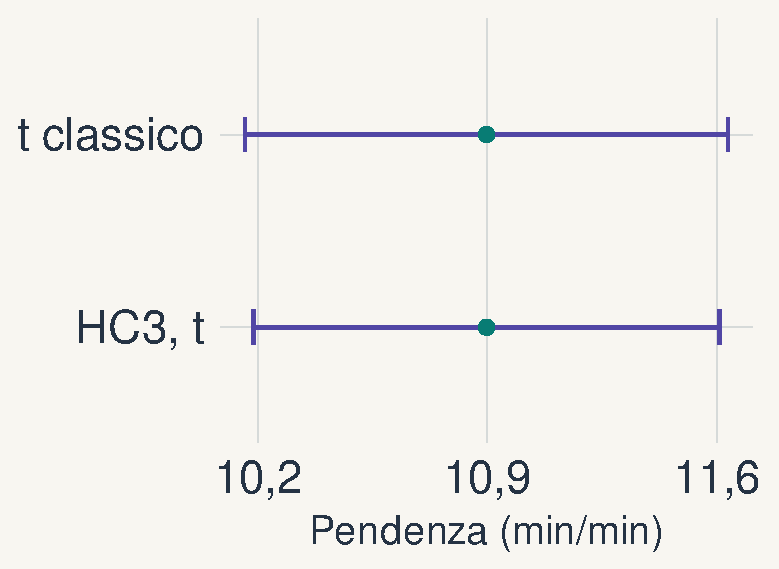
\includegraphics[width=\linewidth,height=6.15cm,keepaspectratio]{Figure/F09.pdf}\par}
\PSmall{Stima OLS comune e due intervalli della pendenza. Per HC3 il riferimento t è approssimativo.}
}};
\node[anchor=north west,inner sep=0] at([xshift=10.85cm,yshift=-2.12cm]current page.north west){\Colonna{8.16cm}{\PBody{L’intervallo t classico al 95\% va da circa 10,161 a 11,635, mentre la costruzione HC3 va da circa 10,188 a 11,608 minuti per minuto. Nel secondo caso si utilizza lo stesso quantile t con 188 gradi di libertà come approssimazione dichiarata. Le ampiezze risultano simili in questo campione, senza che ciò costituisca una prova di omoschedasticità. La vicinanza fra le due costruzioni documenta soltanto una sensibilità limitata alla variante di covarianza effettivamente esaminata.}
}};
\end{tikzpicture}\end{frame}

\begin{frame}[plain]\hypertarget{slide13}{}
\bookmark[level=0,page=13]{Incertezza della media e di un evento}
\bookmark[level=1,page=13]{L’incertezza di un nuovo evento}
\begin{tikzpicture}[remember picture,overlay]
\PilotChrome{L’incertezza di un nuovo evento}{INCERTEZZA DELLA MEDIA E DI UN EVENTO}{13}{La quantità oggetto dell’intervallo deve essere definita prima di interpretarne l’ampiezza.}
\node[anchor=north west,inner sep=0] at([xshift=.96cm,yshift=-2.12cm]current page.north west){\Colonna{9.40cm}{{\centering\resizebox{0.90\linewidth}{!}{\begin{tikzpicture}[x=1cm,y=-.87cm,every node/.style={font=\fontsize{12.2}{15}\selectfont,text=Ink},arr/.style={-{Stealth[length=2mm]},line width=.8pt,draw=Classical}]\path[use as bounding box] (0,0) rectangle (7.45,6.2);
\draw[Rule,line width=.8pt] (0.8,3)--(6.7,3);
\draw[Quantum,line width=.8pt] (1,1.8)--(1,4.2);
\draw[Quantum,line width=.8pt] (6.4,1.8)--(6.4,4.2);
\draw[Classical,line width=.8pt] (2.7,2.4)--(2.7,3.6);
\draw[Classical,line width=.8pt] (4.7,2.4)--(4.7,3.6);
\node[anchor=center,text=Ink,font=\fontsize{11.5}{15}\selectfont,text width=6.5cm,align=center] at (3.7,1) {Nuovo evento: fascia più ampia};
\node[anchor=center,text=Ink,font=\fontsize{11.5}{15}\selectfont,text width=6.5cm,align=center] at (3.7,4.6) {Media condizionata: fascia interna};
\node[anchor=center,text=Ink,font=\fontsize{11}{15}\selectfont,text width=6.6cm,align=center] at (3.7,5.8) {Stesso livello nominale, quantità differenti};

\end{tikzpicture}}\par}
\PSmall{$v_0=(1,x_0)^T$; X: colonne 1 e durata; $\hat y_0$: attesa stimata. $s^2=\sum\hat e_i^2/188$; $t=t_{0,975;188}$.}
}};
\node[anchor=north west,inner sep=0] at([xshift=10.85cm,yshift=-2.12cm]current page.north west){\Colonna{8.16cm}{\PBody{L’intervallo della media descrive l’incertezza sulla posizione della retta a una durata fissata. Per un nuovo evento si aggiunge la variabilità residua individuale, che compare nella formula attraverso il termine uno sotto radice. Entrambe le costruzioni adottano il modello classico omoschedastico e la stessa varianza residua. La covarianza HC3 della pendenza non viene trasformata automaticamente in un intervallo predittivo robusto, poiché quest’ultimo richiederebbe anche un modello della distribuzione del nuovo errore.}
\par\smallskip{\centering\adjustbox{max width=.98\linewidth}{$\displaystyle \begin{gathered}h_0=v_0^T(X^TX)^{-1}v_0\\IC_{\rm media}:\ \hat y_0\pm ts\sqrt{h_0},\quad IP:\ \hat y_0\pm ts\sqrt{1+h_0}\end{gathered}$}\par\smallskip}
}};
\end{tikzpicture}\end{frame}

\begin{frame}[plain]\hypertarget{slide14}{}
\bookmark[level=1,page=14]{Le due fasce vengono lette sulla stessa scala}
\begin{tikzpicture}[remember picture,overlay]
\PilotChrome{Le due fasce vengono lette sulla stessa scala}{INCERTEZZA DELLA MEDIA E DI UN EVENTO}{14}{Una fascia stretta intorno alla retta non implica una previsione individuale altrettanto precisa.}
\node[anchor=north west,inner sep=0] at([xshift=.96cm,yshift=-2.12cm]current page.north west){\Colonna{9.40cm}{{\centering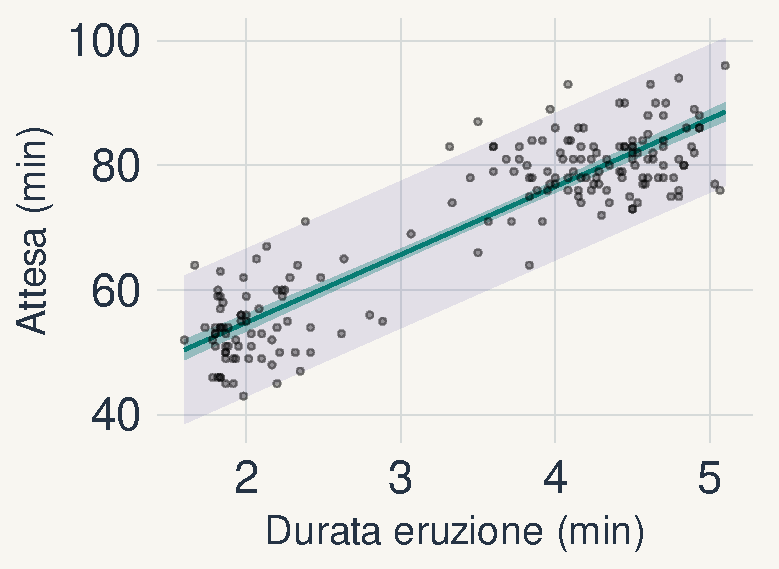
\includegraphics[width=\linewidth,height=6.15cm,keepaspectratio]{Figure/F03.pdf}\par}
\PSmall{Verde: intervallo della media; viola: intervallo predittivo individuale. Costruzioni classiche al 95\%.}
}};
\node[anchor=north west,inner sep=0] at([xshift=10.85cm,yshift=-2.12cm]current page.north west){\Colonna{8.16cm}{\PBody{La fascia verde segue l’incertezza della media condizionata, mentre quella viola rappresenta il nuovo evento sotto le ipotesi classiche. Entrambe si allargano allontanandosi dalla durata media del campione, poiché cresce la leva del punto di previsione. La fascia individuale rimane più ampia per il contributo della variabilità residua. Il disegno viene limitato al dominio delle durate osservate nel campione di adattamento, entro il quale restano comunque zone poco popolate e assunzioni di forma che devono essere discusse.}
}};
\end{tikzpicture}\end{frame}

\begin{frame}[plain]\hypertarget{slide15}{}
\bookmark[level=1,page=15]{I residui precedono l’interpretazione predittiva}
\begin{tikzpicture}[remember picture,overlay]
\PilotChrome{I residui precedono l’interpretazione predittiva}{INCERTEZZA DELLA MEDIA E DI UN EVENTO}{15}{La diagnosi del modello interpreta la struttura residua prima della valutazione sui dati separati.}
\node[anchor=north west,inner sep=0] at([xshift=.96cm,yshift=-2.12cm]current page.north west){\Colonna{9.40cm}{{\centering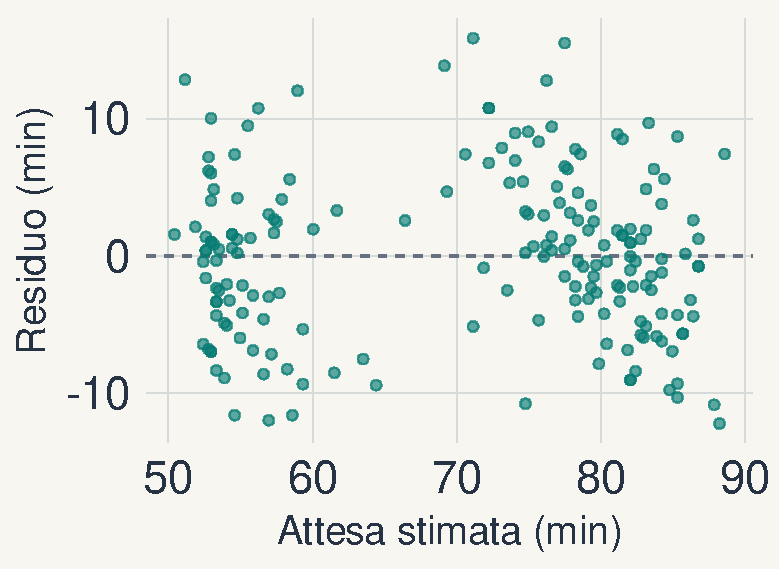
\includegraphics[width=\linewidth,height=6.15cm,keepaspectratio]{Figure/F04.pdf}\par}
\PSmall{Residui dei 190 eventi usati per stimare la retta. Il riferimento tratteggiato indica residuo nullo.}
}};
\node[anchor=north west,inner sep=0] at([xshift=10.85cm,yshift=-2.12cm]current page.north west){\Colonna{8.16cm}{\PBody{Il grafico dei residui rispetto alle attese stimate esamina la forma della relazione e la dispersione rimasta attorno alla retta. Strutture sistematiche potrebbero suggerire curvature, gruppi o variazioni di varianza, mentre punti isolati richiederebbero un controllo della fonte. La diagnosi resta confinata ai dati di adattamento. Le proprietà algebriche dei residui OLS, fra cui l’ortogonalità ai predittori, non garantiscono da sole la forma distributiva dell’errore futuro né la stabilità della relazione fra campagne osservative differenti.}
}};
\end{tikzpicture}\end{frame}

\begin{frame}[plain]\hypertarget{slide16}{}
\bookmark[level=0,page=16]{Valutazione su eventi separati}
\bookmark[level=1,page=16]{La previsione costante usa soltanto l’adattamento}
\begin{tikzpicture}[remember picture,overlay]
\PilotChrome{La previsione costante usa soltanto l’adattamento}{VALUTAZIONE SU EVENTI SEPARATI}{16}{Il riferimento predittivo deve rispettare gli stessi vincoli informativi del modello esaminato.}
\node[anchor=north west,inner sep=0] at([xshift=.96cm,yshift=-2.12cm]current page.north west){\Colonna{9.40cm}{{\centering\resizebox{0.90\linewidth}{!}{\begin{tikzpicture}[x=1cm,y=-.87cm,every node/.style={font=\fontsize{12.2}{15}\selectfont,text=Ink},arr/.style={-{Stealth[length=2mm]},line width=.8pt,draw=Classical}]\path[use as bounding box] (0,0) rectangle (7.45,6.2);
\draw[draw=Classical,fill=Classical!8,rounded corners=2pt,line width=.7pt] (0.5,0.6) rectangle (6.9,1.9);
\node[anchor=center,text=Ink,font=\fontsize{11.5}{15}\selectfont,text width=6cm,align=center] at (3.7,1.25) {Dati di adattamento: media e coefficienti};
\draw[arr,draw=Classical] (2,2.1)--(2,3);
\draw[arr,draw=Quantum] (5.4,2.1)--(5.4,3);
\draw[draw=Classical,fill=Classical!8,rounded corners=2pt,line width=.7pt] (0.4,3.2) rectangle (3.5,4.8);
\node[anchor=center,text=Ink,font=\fontsize{11.5}{15}\selectfont,text width=2.8cm,align=center] at (1.95,4) {Previsione costante};
\draw[draw=Quantum,fill=Quantum!8,rounded corners=2pt,line width=.7pt] (3.9,3.2) rectangle (7,4.8);
\node[anchor=center,text=Ink,font=\fontsize{11.5}{15}\selectfont,text width=2.8cm,align=center] at (5.45,4) {Previsione lineare};
\node[anchor=center,text=Ink,font=\fontsize{11.5}{15}\selectfont,text width=6.7cm,align=center] at (3.7,5.7) {Confronto sugli stessi 82 eventi separati};

\end{tikzpicture}}\par}
\PSmall{$x_i$: durata del nuovo evento; $\bar y_{train}$: attesa media; $\hat\alpha,\hat\beta$: coefficienti. Tutte le stime usano i soli 190 eventi di adattamento.}
}};
\node[anchor=north west,inner sep=0] at([xshift=10.85cm,yshift=-2.12cm]current page.north west){\Colonna{8.16cm}{\PBody{La procedura di riferimento assegna a ogni evento di verifica la media dell’attesa calcolata sui 190 eventi di adattamento, circa 70,479 minuti. Questa scelta stabilisce quanto si guadagni utilizzando la durata rispetto a una previsione priva di predittori. Impiegare la media degli 82 eventi di verifica introdurrebbe informazione della risposta proprio nel riferimento che si intende valutare. Entrambe le procedure vengono quindi definite prima del confronto finale e misurate sulle stesse osservazioni.}
\par\smallskip{\centering\adjustbox{max width=.98\linewidth}{$\displaystyle \widehat y_i^{(0)}=\overline y_{train},\qquad \widehat y_i^{(1)}=\widehat\alpha+\widehat\beta x_i$}\par\smallskip}
}};
\end{tikzpicture}\end{frame}

\begin{frame}[plain]\hypertarget{slide17}{}
\bookmark[level=1,page=17]{La misura dell’errore mantiene il campione separato}
\begin{tikzpicture}[remember picture,overlay]
\PilotChrome{{\fontsize{15.3}{19}\selectfont La misura dell’errore mantiene il campione separato}}{VALUTAZIONE SU EVENTI SEPARATI}{17}{Il test valuta una procedura definita; il suo riutilizzo per scegliere la procedura modifica il disegno.}
\node[anchor=north west,inner sep=0] at([xshift=.96cm,yshift=-2.12cm]current page.north west){\Colonna{9.40cm}{\PBody{Il codice adatta la retta sui dati train e produce previsioni per le durate presenti nel test. Lo scarto fra attesa osservata e prevista viene poi riassunto mediante RMSE e MAE, che attribuiscono peso diverso agli errori grandi. Le misure riguardano gli 82 eventi separati. Una modifica del modello suggerita dai risultati del test richiederebbe un ulteriore campione indipendente per una nuova valutazione finale.}
\par\smallskip{\centering\adjustbox{max width=.98\linewidth}{$\displaystyle \begin{gathered}RMSE=\sqrt{\frac1{82}\sum_i(y_i-\widehat y_i)^2}\\MAE=\frac1{82}\sum_i|y_i-\widehat y_i|\end{gathered}$}\par\smallskip}
\PSmall{$y_i$: attesa osservata; $\hat y_i$: previsione, per i = 1,…,82 nel test. RMSE e MAE sono entrambe in minuti.}
}};
\node[anchor=north west,inner sep=0] at([xshift=10.85cm,yshift=-2.12cm]current page.north west){\Colonna{8.16cm}{\begin{tcolorbox}[enhanced,arc=1.7mm,boxrule=.6pt,colback=white,colframe=Classical!60!Navy,colbacktitle=Navy,coltitle=white,fonttitle=\bfseries\small,title={R · calcolo riproducibile},left=1.7mm,right=1.3mm,top=1.1mm,bottom=1.1mm,before skip=1mm,after skip=1.0mm]\lstinputlisting[style=GeoR,language=R,basicstyle=\ttfamily\fontsize{8.6}{11.4}\selectfont]{Codice/previsione.R}\end{tcolorbox}
\PLabel{Risultato in R}
\begin{tcolorbox}[colback=GeoTint,colframe=Rule,boxrule=.5pt,arc=1.4mm,left=2mm,right=1mm,top=1mm,bottom=1mm]{\fontsize{8.4}{10.9}\selectfont\ttfamily \mbox{[1]\ 5.849674}}\end{tcolorbox}
}};
\end{tikzpicture}\end{frame}

\begin{frame}[plain]\hypertarget{slide18}{}
\bookmark[level=1,page=18]{Osservato e previsto rendono visibili gli scarti}
\begin{tikzpicture}[remember picture,overlay]
\PilotChrome{Osservato e previsto rendono visibili gli scarti}{VALUTAZIONE SU EVENTI SEPARATI}{18}{La valutazione predittiva richiede errori espressi nella scala della risposta, oltre all’associazione grafica.}
\node[anchor=north west,inner sep=0] at([xshift=.96cm,yshift=-2.12cm]current page.north west){\Colonna{9.40cm}{{\centering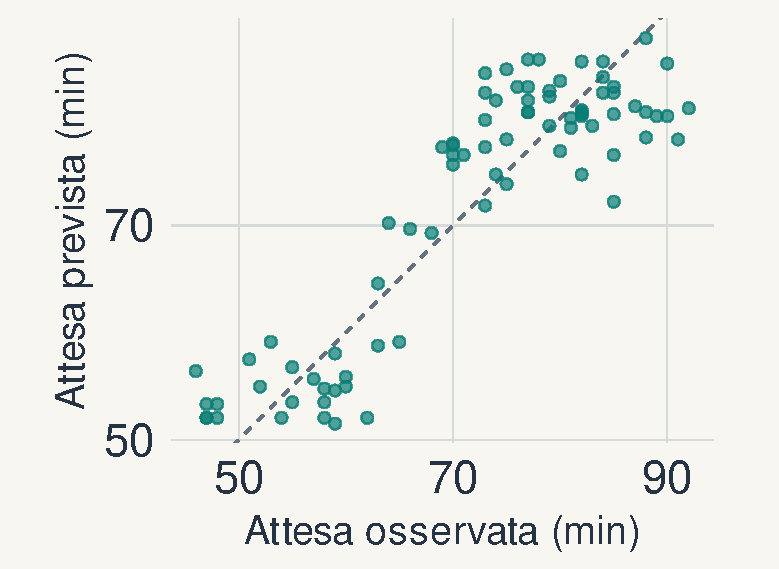
\includegraphics[width=\linewidth,height=6.15cm,keepaspectratio]{Figure/F05.pdf}\par}
\PSmall{Ottantadue eventi di verifica. Bisettrice: previsione uguale all’osservazione; rapporto unitario fra gli assi.}
}};
\node[anchor=north west,inner sep=0] at([xshift=10.85cm,yshift=-2.12cm]current page.north west){\Colonna{8.16cm}{\PBody{Il diagramma confronta ogni attesa osservata con la previsione corrispondente, adottando la stessa scala sui due assi. La bisettrice rappresenta previsione esatta, mentre la distanza verticale rende leggibili sovrastime e sottostime. La presenza dei due addensamenti resta visibile anche negli eventi separati. Una correlazione elevata fra osservato e previsto sarebbe insufficiente a descrivere accuratezza e calibrazione, poiché potrebbe convivere con errori sistematici; per questo il confronto viene accompagnato da misure nella scala dei minuti.}
}};
\end{tikzpicture}\end{frame}

\begin{frame}[plain]\hypertarget{slide19}{}
\bookmark[level=1,page=19]{Il miglioramento viene quantificato in minuti}
\begin{tikzpicture}[remember picture,overlay]
\PilotChrome{Il miglioramento viene quantificato in minuti}{VALUTAZIONE SU EVENTI SEPARATI}{19}{Il guadagno predittivo viene espresso rispetto a un riferimento e a un dominio di valutazione dichiarati.}
\node[anchor=north west,inner sep=0] at([xshift=.96cm,yshift=-2.12cm]current page.north west){\Colonna{9.40cm}{{\centering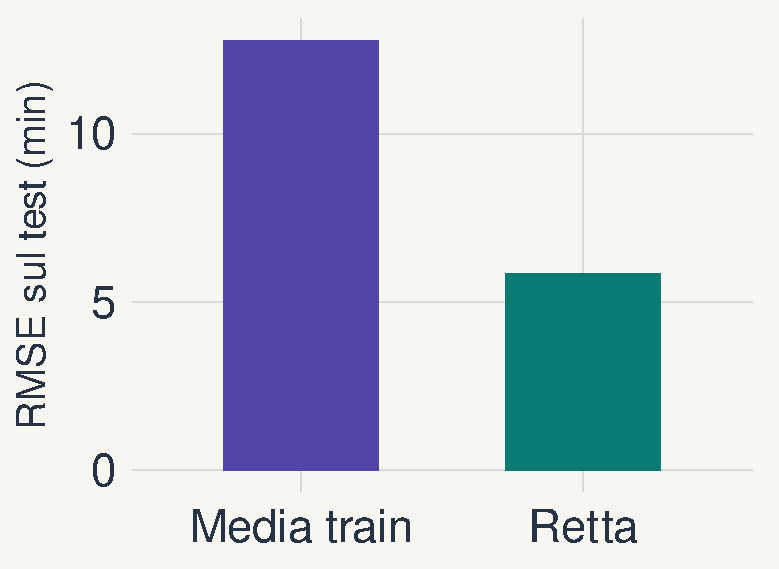
\includegraphics[width=\linewidth,height=6.15cm,keepaspectratio]{Figure/F06.pdf}\par}
\PSmall{RMSE calcolata sugli stessi 82 eventi. La media di riferimento proviene esclusivamente dal train.}
}};
\node[anchor=north west,inner sep=0] at([xshift=10.85cm,yshift=-2.12cm]current page.north west){\Colonna{8.16cm}{\PBody{Sul campione di verifica, la RMSE della previsione costante è circa 12,768 minuti, mentre quella della retta è circa 5,850 minuti. La MAE passa rispettivamente da circa 11,016 a 4,941 minuti. La durata fornisce quindi informazione predittiva utile entro questo esperimento e la separazione dichiarata. La grandezza del miglioramento rimane riferita a questi eventi e alle condizioni di scambiabilità, mentre la valutazione di utilità operativa richiederebbe soglie di errore rilevanti e dati cronologici nuovi.}
}};
\end{tikzpicture}\end{frame}

\begin{frame}[plain]\hypertarget{slide20}{}
\bookmark[level=1,page=20]{La copertura viene osservata nel test}
\begin{tikzpicture}[remember picture,overlay]
\PilotChrome{La copertura viene osservata nel test}{VALUTAZIONE SU EVENTI SEPARATI}{20}{La copertura nominale è una proprietà della procedura sotto ipotesi; quella osservata è una proporzione campionaria.}
\node[anchor=north west,inner sep=0] at([xshift=.96cm,yshift=-2.12cm]current page.north west){\Colonna{9.40cm}{{\centering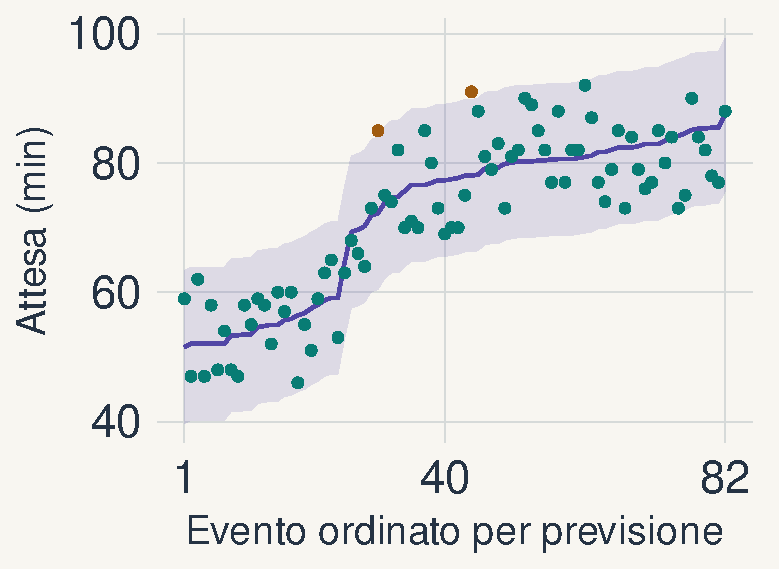
\includegraphics[width=\linewidth,height=6.15cm,keepaspectratio]{Figure/F08.pdf}\par}
\PSmall{$L_i,U_i$: estremi predittivi; $y_i$: attesa osservata. Eventi ordinati per previsione, senza cronologia; ocra: due casi esterni.}
}};
\node[anchor=north west,inner sep=0] at([xshift=10.85cm,yshift=-2.12cm]current page.north west){\Colonna{8.16cm}{\PBody{Ottanta delle ottantadue attese ricadono nei rispettivi intervalli predittivi classici al 95\%, producendo una copertura osservata di circa 97,56\%. La figura ordina gli eventi per previsione e rende riconoscibili le due osservazioni esterne alla fascia. Questa proporzione costituisce una verifica empirica su un campione limitato, soggetta a variabilità e alle condizioni della separazione. La vicinanza al livello nominale non garantisce la medesima copertura per eventi futuri acquisiti con protocolli o condizioni del sistema differenti.}
\par\smallskip{\centering\adjustbox{max width=.98\linewidth}{$\displaystyle \widehat C=\frac1{82}\sum_i\mathbf1\{L_i\leq y_i\leq U_i\}=\frac{80}{82}$}\par\smallskip}
}};
\end{tikzpicture}\end{frame}

\begin{frame}[plain]\hypertarget{slide21}{}
\bookmark[level=0,page=21]{Struttura interna e discussione}
\bookmark[level=1,page=21]{Le pendenze interne differiscono da quella globale}
\begin{tikzpicture}[remember picture,overlay]
\PilotChrome{Le pendenze interne differiscono da quella globale}{STRUTTURA INTERNA E DISCUSSIONE}{21}{L’associazione complessiva può riflettere sia variazioni interne sia differenze fra gruppi.}
\node[anchor=north west,inner sep=0] at([xshift=.96cm,yshift=-2.12cm]current page.north west){\Colonna{9.40cm}{{\centering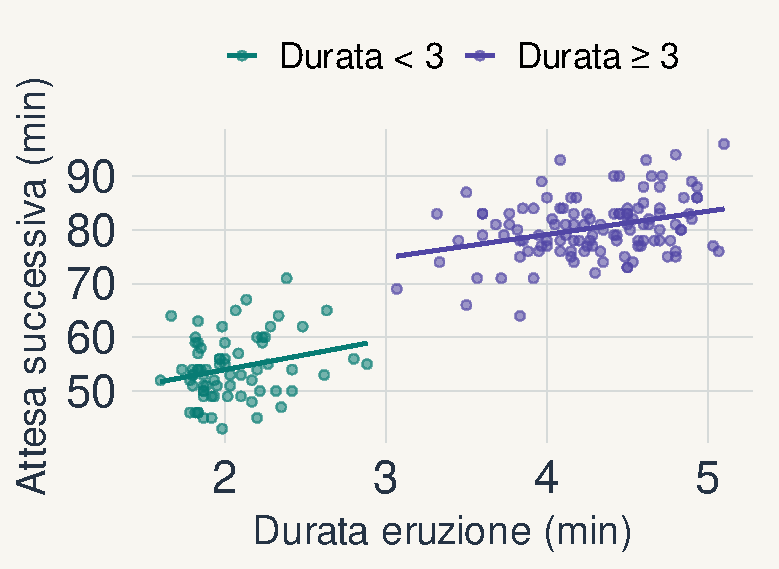
\includegraphics[width=\linewidth,height=6.15cm,keepaspectratio]{Figure/F07.pdf}\par}
\PSmall{Rette entro due intervalli di durata, sul solo train. La soglia di tre minuti è un criterio descrittivo dichiarato.}
}};
\node[anchor=north west,inner sep=0] at([xshift=10.85cm,yshift=-2.12cm]current page.north west){\Colonna{8.16cm}{\PBody{Dividendo il solo campione di adattamento alla durata didattica di tre minuti, le pendenze risultano circa 5,588 e 4,328 nei gruppi di 72 e 118 eventi. Entrambe sono inferiori alla pendenza globale, circa 10,898, che incorpora anche la separazione fra addensamenti. Il confronto descrive una sensibilità dell’associazione e non assegna automaticamente uno stato fisico ai due gruppi. La soglia non viene scelta attraverso il test e le rette separate non sostituiscono retroattivamente la procedura già valutata.}
}};
\end{tikzpicture}\end{frame}

\begin{frame}[plain]\hypertarget{slide22}{}
\bookmark[level=1,page=22]{Consegna: distinguere effetto medio e previsione}
\begin{tikzpicture}[remember picture,overlay]
\PilotChrome{Consegna: distinguere effetto medio e previsione}{STRUTTURA INTERNA E DISCUSSIONE}{22}{La forza della conclusione deriva dal collegamento fra bersaglio, informazione disponibile e disegno della verifica.}
\node[anchor=north west,inner sep=0] at([xshift=.96cm,yshift=-2.12cm]current page.north west){\Colonna{9.40cm}{\PBody{La relazione presenta fonte, separazione, grafici del train, pendenza con intervalli, residui, confronto predittivo e copertura. L’esercizio chiede quale intervallo utilizzare per la media degli eventi a una durata fissata e quale per un singolo nuovo evento, motivando il termine aggiuntivo nella varianza. Una seconda discussione identifica la fuga di informazione introdotta dalla media del test. La conclusione mantiene distinti associazione nel campione, generalizzazione interna e requisiti di una previsione cronologica applicata al sistema reale.}
}};
\node[anchor=north west,inner sep=0] at([xshift=10.85cm,yshift=-2.12cm]current page.north west){\Colonna{8.16cm}{\PInfo{R/P04\_figure.R conserva le previsioni per identificativo e i calcoli della covarianza HC3. I dati e il piano di separazione si trovano in dati/progetti. Il progetto raccorda regressione, intervalli predittivi e validazione dei moduli M07, M10 e M16.}
}};
\end{tikzpicture}\end{frame}

\begin{frame}[plain]\hypertarget{slide23}{}
\bookmark[level=0,page=23]{Laboratori della spedizione}
\bookmark[level=1,page=23]{Tre fasi della spedizione nel laboratorio}
\begin{tikzpicture}[remember picture,overlay]
\PilotChrome{Tre fasi della spedizione nel laboratorio}{LABORATORI DELLA SPEDIZIONE}{23}{Gli esperimenti usano dati sintetici; la conclusione sul caso resta quella ottenuta dagli eventi di faithful.}
\node[anchor=north west,inner sep=0] at([xshift=.96cm,yshift=-2.12cm]current page.north west){\Colonna{9.40cm}{{\centering\resizebox{0.97\linewidth}{!}{\begin{tikzpicture}[x=1cm,y=1cm,every node/.style={font=\sffamily\fontsize{9.2}{11}\selectfont,text=Ink}]
\node[draw=Classical,fill=Classical,rounded corners=2mm,text=white,text width=2.45cm,align=flush center,minimum height=1.55cm,anchor=west,font=\sffamily\bfseries\fontsize{9.2}{11}\selectfont] (f0) at (0,0.00) {1. Separare stima e verifica};
\node[draw=Classical!60,fill=Classical!6,rounded corners=1.5mm,line width=.6pt,text width=2.8cm,align=flush center,minimum height=1.55cm,anchor=west] (e00) at (2.95,0.00) {Complessità e prestazione su nuovi dati\\[1pt]{\fontsize{7.6}{9}\selectfont\color{Muted}m07-validazione}};
\node[draw=Rule,fill=white,rounded corners=1.5mm,line width=.6pt,text width=2.8cm,align=flush center,minimum height=1.55cm,anchor=west] (e01) at (6.10,0.00) {Dominio osservato ed estrapolazione\\[1pt]{\fontsize{7.6}{9}\selectfont\color{Muted}m07-dominio}};
\draw[pEdge] (f0.east)--(e00.west);
\node[draw=Classical,fill=Classical,rounded corners=2mm,text=white,text width=2.45cm,align=flush center,minimum height=1.55cm,anchor=west,font=\sffamily\bfseries\fontsize{9.2}{11}\selectfont] (f1) at (0,-1.95) {2. Costruire il modello};
\draw[pEdge] (f0.south)--(f1.north);
\node[draw=Classical!60,fill=Classical!6,rounded corners=1.5mm,line width=.6pt,text width=2.8cm,align=flush center,minimum height=1.55cm,anchor=west] (e10) at (2.95,-1.95) {La geometria dei minimi quadrati\\[1pt]{\fontsize{7.6}{9}\selectfont\color{Muted}m07-minimi-quadrati}};
\node[draw=Rule,fill=white,rounded corners=1.5mm,line width=.6pt,text width=2.8cm,align=flush center,minimum height=1.55cm,anchor=west] (e11) at (6.10,-1.95) {Leva e influenza di un’osservazione\\[1pt]{\fontsize{7.6}{9}\selectfont\color{Muted}m07-influenza}};
\draw[pEdge] (f1.east)--(e10.west);
\node[draw=Classical,fill=Classical,rounded corners=2mm,text=white,text width=2.45cm,align=flush center,minimum height=1.55cm,anchor=west,font=\sffamily\bfseries\fontsize{9.2}{11}\selectfont] (f2) at (0,-3.90) {3. Interpretare le previsioni};
\draw[pEdge] (f1.south)--(f2.north);
\node[draw=Classical!60,fill=Classical!6,rounded corners=1.5mm,line width=.6pt,text width=2.8cm,align=flush center,minimum height=1.55cm,anchor=west] (e20) at (2.95,-3.90) {Intervallo della media e di una nuova osservazione\\[1pt]{\fontsize{7.6}{9}\selectfont\color{Muted}m07-previsione}};
\node[draw=Rule,fill=white,rounded corners=1.5mm,line width=.6pt,text width=2.8cm,align=flush center,minimum height=1.55cm,anchor=west] (e21) at (6.10,-3.90) {Effetto, intervallo ed evidenza\\[1pt]{\fontsize{7.6}{9}\selectfont\color{Muted}m06-relazione}};
\draw[pEdge] (f2.east)--(e20.west);
\end{tikzpicture}
}\par}
\PSmall{Fasi della spedizione. Il primo esperimento di ogni fase ha le pagine Scenario A e Confronto.}
}};
\node[anchor=north west,inner sep=0] at([xshift=10.85cm,yshift=-2.12cm]current page.north west){\Colonna{8.16cm}{\PBody{Gli esperimenti ripetono su dati sintetici tre passaggi della spedizione: separare stima e verifica, costruire la retta dei minimi quadrati, distinguere l’intervallo della media da quello di una nuova osservazione. Ogni fase ha uno scenario di partenza e un confronto con un solo parametro modificato.}
\vspace{.2cm}\PLabel{Altri esperimenti delle fasi}
\PLab{https://marzione00.github.io/Lab_Geo/\#laboratorio/m07-dominio}{Dominio osservato ed estrapolazione · m07-dominio}
\PLab{https://marzione00.github.io/Lab_Geo/\#laboratorio/m07-influenza}{Leva e influenza di un’osservazione · m07-influenza}
\PLab{https://marzione00.github.io/Lab_Geo/\#laboratorio/m06-relazione}{Effetto, intervallo ed evidenza · m06-relazione}
}};
\end{tikzpicture}\end{frame}

\begin{frame}[plain]\hypertarget{slide24}{}
\bookmark[level=1,page=24]{Complessità e prestazione su nuovi dati}
\begin{tikzpicture}[remember picture,overlay]
\PilotChrome{Complessità e prestazione su nuovi dati}{LABORATORI DELLA SPEDIZIONE}{24}{Confrontare errore di adattamento e di previsione.}
\node[anchor=north west,inner sep=0] at([xshift=.96cm,yshift=-2.12cm]current page.north west){\Colonna{9.40cm}{{\centering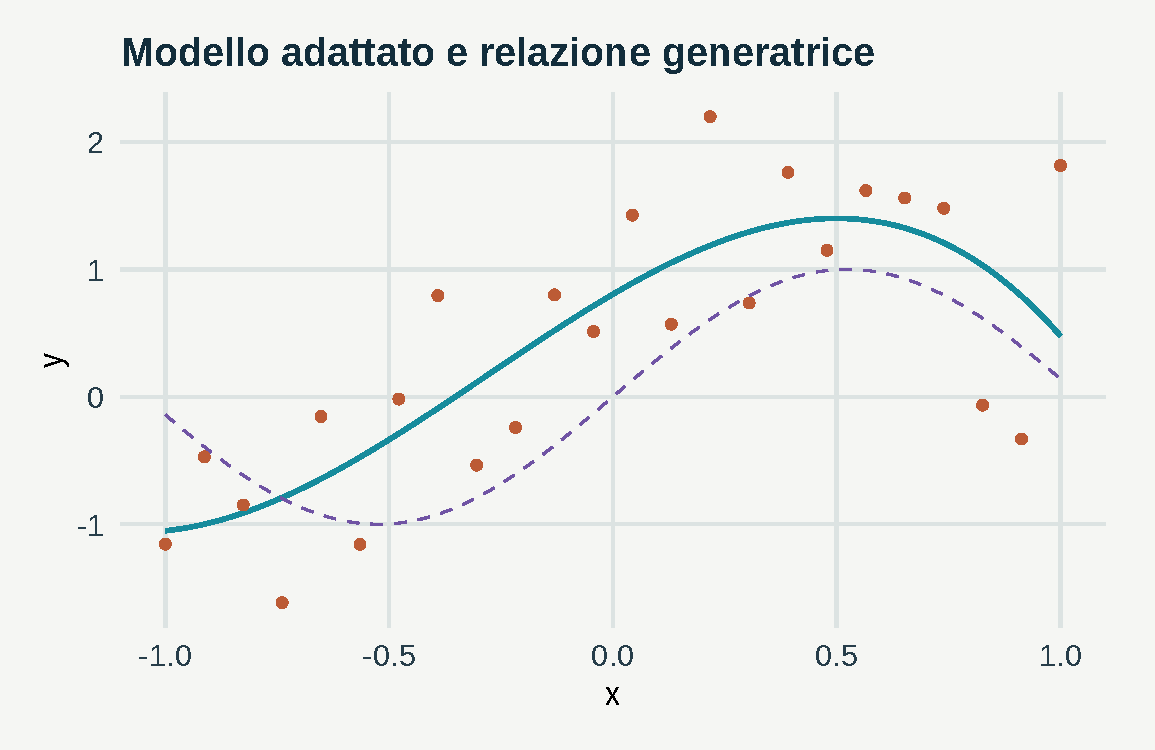
\includegraphics[width=\linewidth,height=5.0cm,keepaspectratio]{Esperimenti/m07-validazione-A.pdf}\par}
\PSmall{Grado del polinomio: 3. Seme: 17.}
\PSmall{$y_i$ è la risposta osservata nel campione di verifica; $\widehat y_i$ è la previsione del modello; $m$ conta le osservazioni valutate. RMSE è la radice dell’errore quadratico medio e mantiene l’unità della risposta.}
}};
\node[anchor=north west,inner sep=0] at([xshift=10.85cm,yshift=-2.12cm]current page.north west){\Colonna{8.16cm}{\PLabel{Scenario A · simulazione}
\PBody{Un campione rumoroso di una relazione sinusoidale viene utilizzato per adattare polinomi di grado crescente. Un secondo insieme di risposte, generato separatamente sullo stesso dominio, permette di valutare la previsione su osservazioni nuove. Mantenendo il seme, le modifiche al grado confrontano modelli diversi applicati ai medesimi dati.}
\par\smallskip{\centering\adjustbox{max width=.98\linewidth}{$\displaystyle \operatorname{RMSE}=\sqrt{m^{-1}\sum_{i=1}^{m}(y_i-\widehat y_i)^2}$}\par\smallskip}
}};
\node[anchor=north east,inner sep=0] at([xshift=17.1cm,yshift=-12.04cm]current page.north west){\fontsize{7.7}{9}\selectfont \href{https://marzione00.github.io/Lab_Geo/\#laboratorio/m07-validazione}{\color{Classical}\bfseries Apri il laboratorio · m07-validazione}};
\end{tikzpicture}\end{frame}

\begin{frame}[plain]\hypertarget{slide25}{}
\bookmark[level=1,page=25]{Confronto | Complessità e prestazione su nuovi dati}
\begin{tikzpicture}[remember picture,overlay]
\PilotChrome{{\fontsize{15.3}{19}\selectfont Confronto | Complessità e prestazione su nuovi dati}}{LABORATORI DELLA SPEDIZIONE}{25}{L’errore sul campione di adattamento può diminuire mentre quello su nuove osservazioni aumenta.}
\node[anchor=north west,inner sep=0] at([xshift=.96cm,yshift=-2.12cm]current page.north west){\Colonna{9.40cm}{{\centering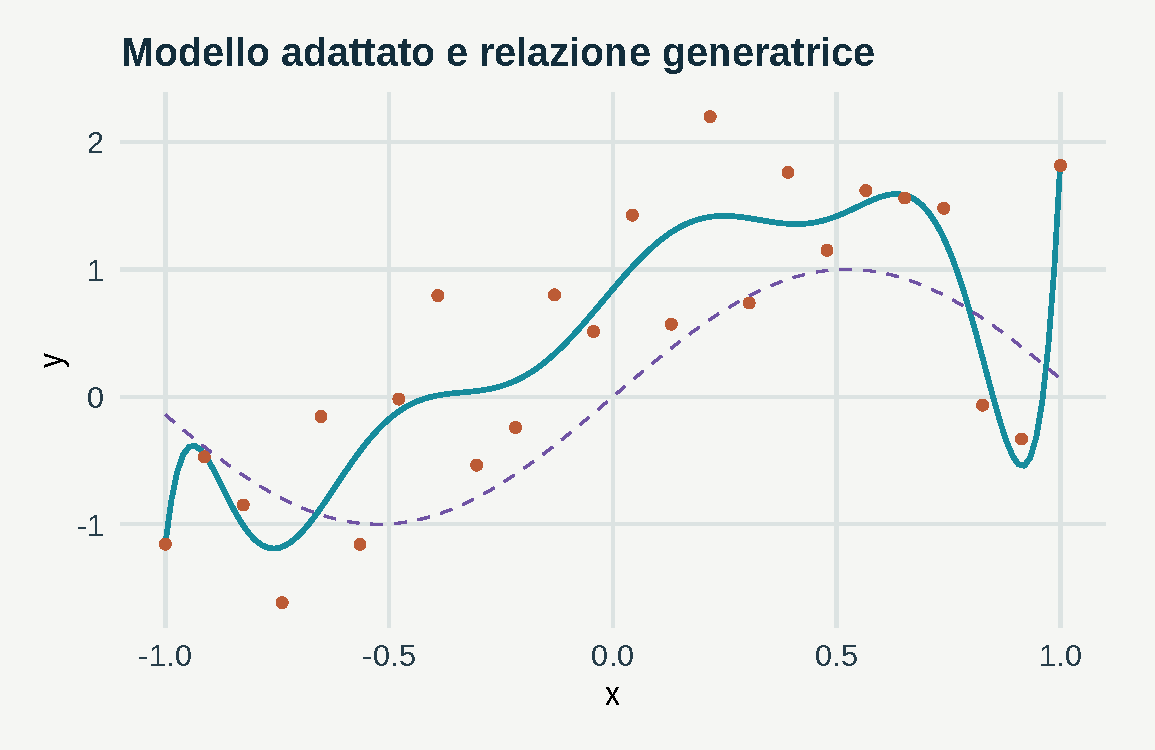
\includegraphics[width=\linewidth,height=5.6cm,keepaspectratio]{Esperimenti/m07-validazione-B.pdf}\par}
\PSmall{Grado del polinomio: 3 $\to$ 9. Tutti gli altri parametri e il seme sono fissi.}
}};
\node[anchor=north west,inner sep=0] at([xshift=10.85cm,yshift=-2.12cm]current page.north west){\Colonna{8.16cm}{\PLabel{Confronto fra gli scenari}
{\fontsize{10.2}{12.8}\selectfont\begin{tabular}{@{}>{\raggedright\arraybackslash}p{0.48\linewidth}@{\hspace{.13cm}}>{\raggedright\arraybackslash}p{0.224\linewidth}@{\hspace{.13cm}}>{\raggedright\arraybackslash}p{0.224\linewidth}@{}}\toprule Grandezza & A & B\\[2.3pt]
\midrule 
RMSE adattamento & 0,642 & 0,448\\[2.3pt]
RMSE nuove osservazioni & 1,28 & 1,3\\[2.3pt]
\bottomrule\end{tabular}\par}
\vspace{.25cm}\PBody{Con un polinomio di grado nove l’errore sui dati di adattamento scende da 0,642 a 0,448, mentre quello sulle nuove osservazioni passa da 1,28 a 1,3. La complessità migliora l’aderenza al campione e lascia invariata la qualità della previsione.}
}};
\node[anchor=north east,inner sep=0] at([xshift=17.1cm,yshift=-12.04cm]current page.north west){\fontsize{7.7}{9}\selectfont \href{https://marzione00.github.io/Lab_Geo/\#laboratorio/m07-validazione}{\color{Classical}\bfseries Apri il laboratorio · m07-validazione}};
\end{tikzpicture}\end{frame}

\begin{frame}[plain]\hypertarget{slide26}{}
\bookmark[level=1,page=26]{La geometria dei minimi quadrati}
\begin{tikzpicture}[remember picture,overlay]
\PilotChrome{La geometria dei minimi quadrati}{LABORATORI DELLA SPEDIZIONE}{26}{Confrontare una retta proposta con la soluzione che minimizza gli scarti quadratici.}
\node[anchor=north west,inner sep=0] at([xshift=.96cm,yshift=-2.12cm]current page.north west){\Colonna{9.40cm}{{\centering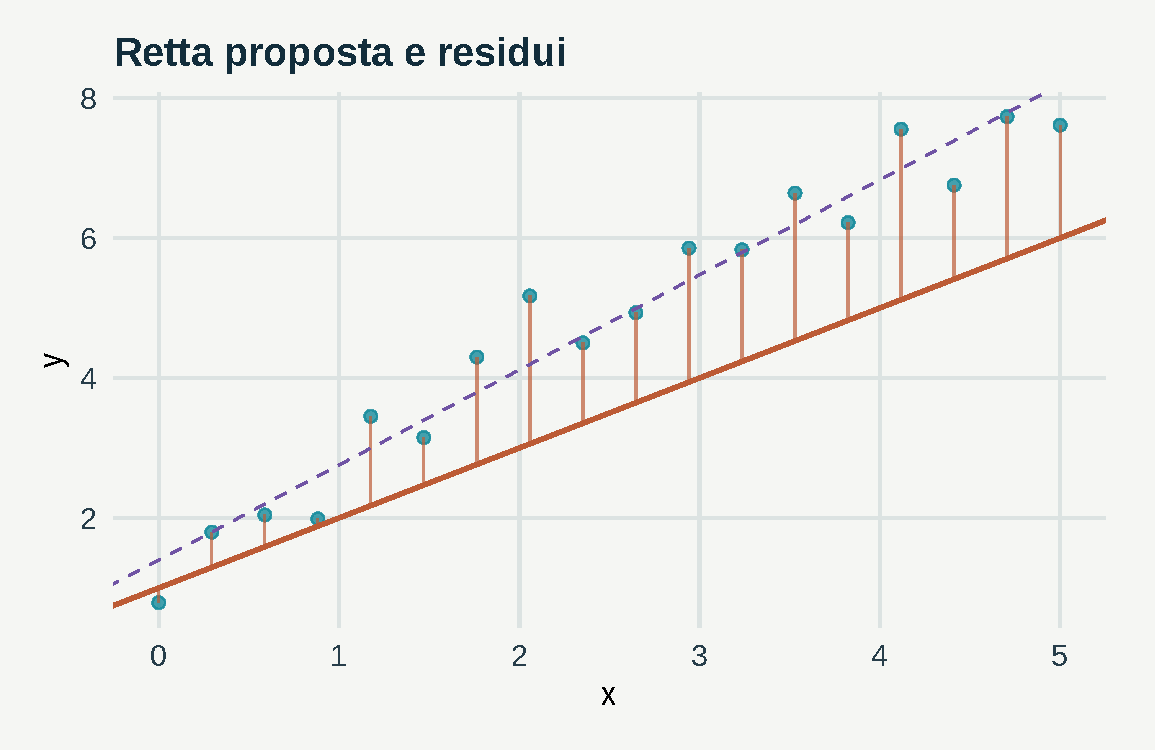
\includegraphics[width=\linewidth,height=5.0cm,keepaspectratio]{Esperimenti/m07-minimi-quadrati-A.pdf}\par}
\PSmall{Pendenza proposta: 1. Seme: 17.}
\PSmall{$x_i$ e $y_i$ sono predittore e risposta osservati; $a$ e $b$ sono intercetta e pendenza candidate. $\widehat\beta_0$ e $\widehat\beta_1$ identificano la coppia che minimizza la somma dei residui al quadrato.}
}};
\node[anchor=north west,inner sep=0] at([xshift=10.85cm,yshift=-2.12cm]current page.north west){\Colonna{8.16cm}{\PLabel{Scenario A · simulazione}
\PBody{Una retta proposta assegna a ogni valore del predittore una risposta prevista. I segmenti verticali collegano ciascuna osservazione alla previsione corrispondente e rappresentano i residui. Modificando intercetta e pendenza si osserva come questi scarti cambino simultaneamente e come la loro somma quadratica misuri la qualità dell’adattamento al campione.}
\par\smallskip{\centering\adjustbox{max width=.98\linewidth}{$\displaystyle (\widehat\beta_0,\widehat\beta_1)=\arg\min_{a,b}\sum_i(y_i-a-bx_i)^2$}\par\smallskip}
}};
\node[anchor=north east,inner sep=0] at([xshift=17.1cm,yshift=-12.04cm]current page.north west){\fontsize{7.7}{9}\selectfont \href{https://marzione00.github.io/Lab_Geo/\#laboratorio/m07-minimi-quadrati}{\color{Classical}\bfseries Apri il laboratorio · m07-minimi-quadrati}};
\end{tikzpicture}\end{frame}

\begin{frame}[plain]\hypertarget{slide27}{}
\bookmark[level=1,page=27]{Confronto | La geometria dei minimi quadrati}
\begin{tikzpicture}[remember picture,overlay]
\PilotChrome{Confronto | La geometria dei minimi quadrati}{LABORATORI DELLA SPEDIZIONE}{27}{La soluzione OLS minimizza la somma dei quadrati sul campione dichiarato.}
\node[anchor=north west,inner sep=0] at([xshift=.96cm,yshift=-2.12cm]current page.north west){\Colonna{9.40cm}{{\centering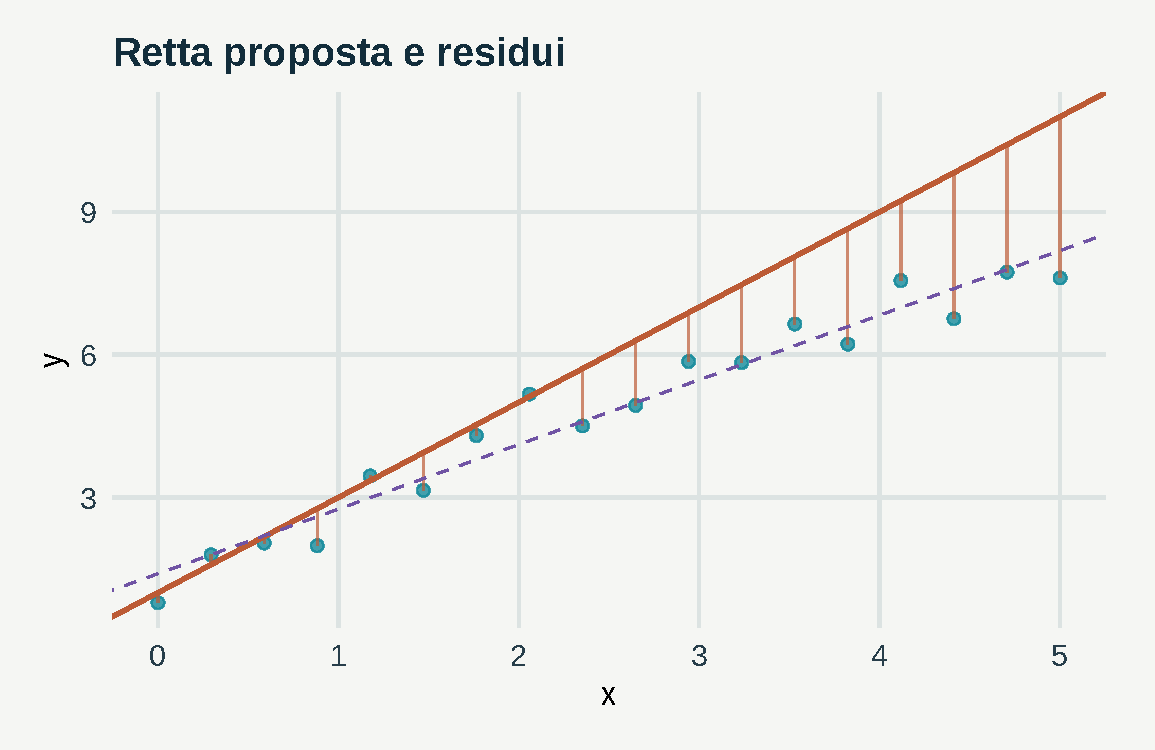
\includegraphics[width=\linewidth,height=5.6cm,keepaspectratio]{Esperimenti/m07-minimi-quadrati-B.pdf}\par}
\PSmall{Pendenza proposta: 1 $\to$ 2. Tutti gli altri parametri e il seme sono fissi.}
}};
\node[anchor=north west,inner sep=0] at([xshift=10.85cm,yshift=-2.12cm]current page.north west){\Colonna{8.16cm}{\PLabel{Confronto fra gli scenari}
{\fontsize{10.2}{12.8}\selectfont\begin{tabular}{@{}>{\raggedright\arraybackslash}p{0.48\linewidth}@{\hspace{.13cm}}>{\raggedright\arraybackslash}p{0.224\linewidth}@{\hspace{.13cm}}>{\raggedright\arraybackslash}p{0.224\linewidth}@{}}\toprule Grandezza & A & B\\[2.3pt]
\midrule 
SSE proposta & 39,5 & 47,2\\[2.3pt]
SSE minima OLS & 3,87 & 3,87\\[2.3pt]
Intercetta OLS & 1,4 & 1,4\\[2.3pt]
Pendenza OLS & 1,36 & 1,36\\[2.3pt]
\bottomrule\end{tabular}\par}
\vspace{.25cm}\PBody{Con pendenza proposta 2 la somma dei quadrati dei residui passa da 39,5 a 47,2, mentre il minimo dei minimi quadrati resta 3,87 con intercetta 1,4 e pendenza 1,36. La retta proposta cambia l’errore; la soluzione ottima dipende soltanto dai dati.}
}};
\node[anchor=north east,inner sep=0] at([xshift=17.1cm,yshift=-12.04cm]current page.north west){\fontsize{7.7}{9}\selectfont \href{https://marzione00.github.io/Lab_Geo/\#laboratorio/m07-minimi-quadrati}{\color{Classical}\bfseries Apri il laboratorio · m07-minimi-quadrati}};
\end{tikzpicture}\end{frame}

\begin{frame}[plain]\hypertarget{slide28}{}
\bookmark[level=1,page=28]{Intervallo della media e di una nuova osservazione}
\begin{tikzpicture}[remember picture,overlay]
\PilotChrome{Intervallo della media e di una nuova osservazione}{LABORATORI DELLA SPEDIZIONE}{28}{Separare incertezza della risposta media e variabilità di un evento futuro.}
\node[anchor=north west,inner sep=0] at([xshift=.96cm,yshift=-2.12cm]current page.north west){\Colonna{9.40cm}{{\centering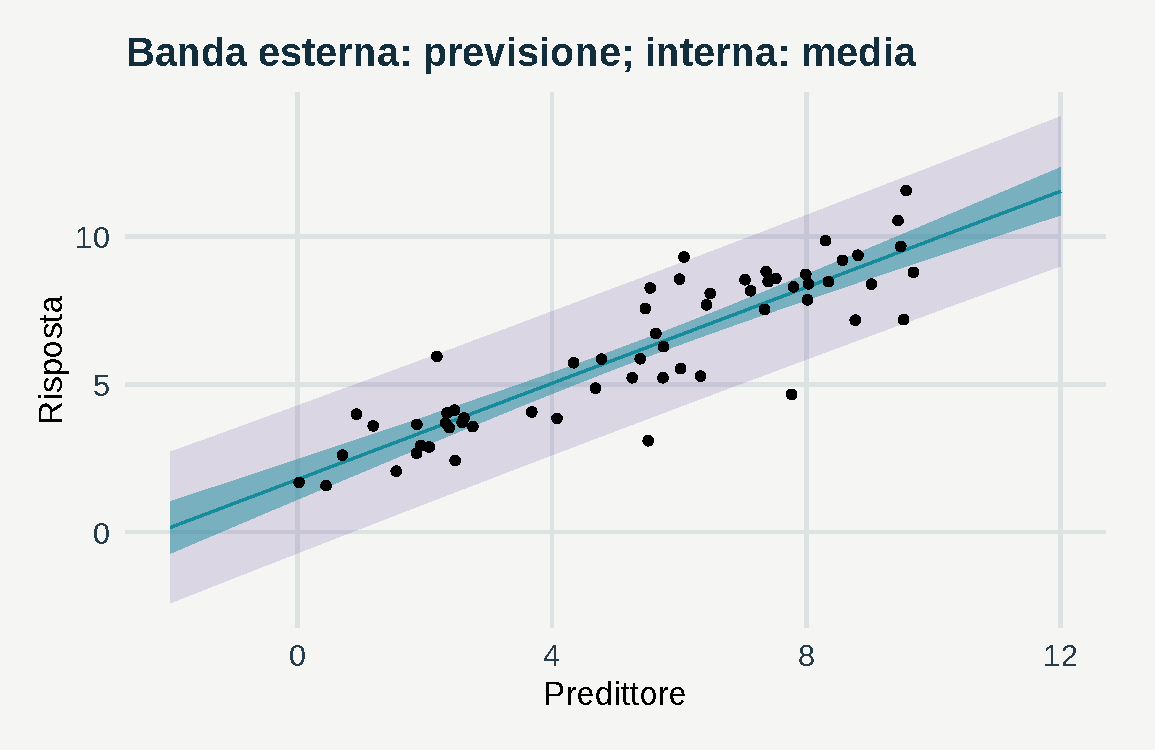
\includegraphics[width=\linewidth,height=5.0cm,keepaspectratio]{Esperimenti/m07-previsione-A.pdf}\par}
\PSmall{Numero di osservazioni: 60. Seme: 17.}
\PSmall{$x_0$ è la posizione considerata; $s$ è la deviazione standard residua stimata; $h_0$ misura l’incertezza geometrica della media in $x_0$. $\operatorname{SE}_{media}$ riguarda la risposta media, mentre $\operatorname{SE}_{pred}$ include una nuova osservazione.}
}};
\node[anchor=north west,inner sep=0] at([xshift=10.85cm,yshift=-2.12cm]current page.north west){\Colonna{8.16cm}{\PLabel{Scenario A · simulazione}
\PBody{Il campione proviene da una relazione lineare con errori normali indipendenti e varianza costante. Dopo l’adattamento della retta, vengono costruiti un intervallo per la risposta media e uno per una nuova osservazione in ogni posizione del predittore. Il secondo comprende sia l’incertezza della media stimata sia la variabilità individuale residua.}
\par\smallskip{\centering\adjustbox{max width=.98\linewidth}{$\displaystyle \operatorname{SE}_{pred}(x_0)=s\sqrt{1+h_0},\quad\operatorname{SE}_{media}(x_0)=s\sqrt{h_0}$}\par\smallskip}
}};
\node[anchor=north east,inner sep=0] at([xshift=17.1cm,yshift=-12.04cm]current page.north west){\fontsize{7.7}{9}\selectfont \href{https://marzione00.github.io/Lab_Geo/\#laboratorio/m07-previsione}{\color{Classical}\bfseries Apri il laboratorio · m07-previsione}};
\end{tikzpicture}\end{frame}

\begin{frame}[plain]\hypertarget{slide29}{}
\bookmark[level=1,page=29]{Confronto | Intervallo della media e di una nuova osservazione}
\begin{tikzpicture}[remember picture,overlay]
\PilotChrome{{\fontsize{15.3}{19}\selectfont Confronto | Intervallo della media e di una nuova osservazione}}{LABORATORI DELLA SPEDIZIONE}{29}{L’intervallo di previsione comprende anche la variabilità di una nuova osservazione.}
\node[anchor=north west,inner sep=0] at([xshift=.96cm,yshift=-2.12cm]current page.north west){\Colonna{9.40cm}{{\centering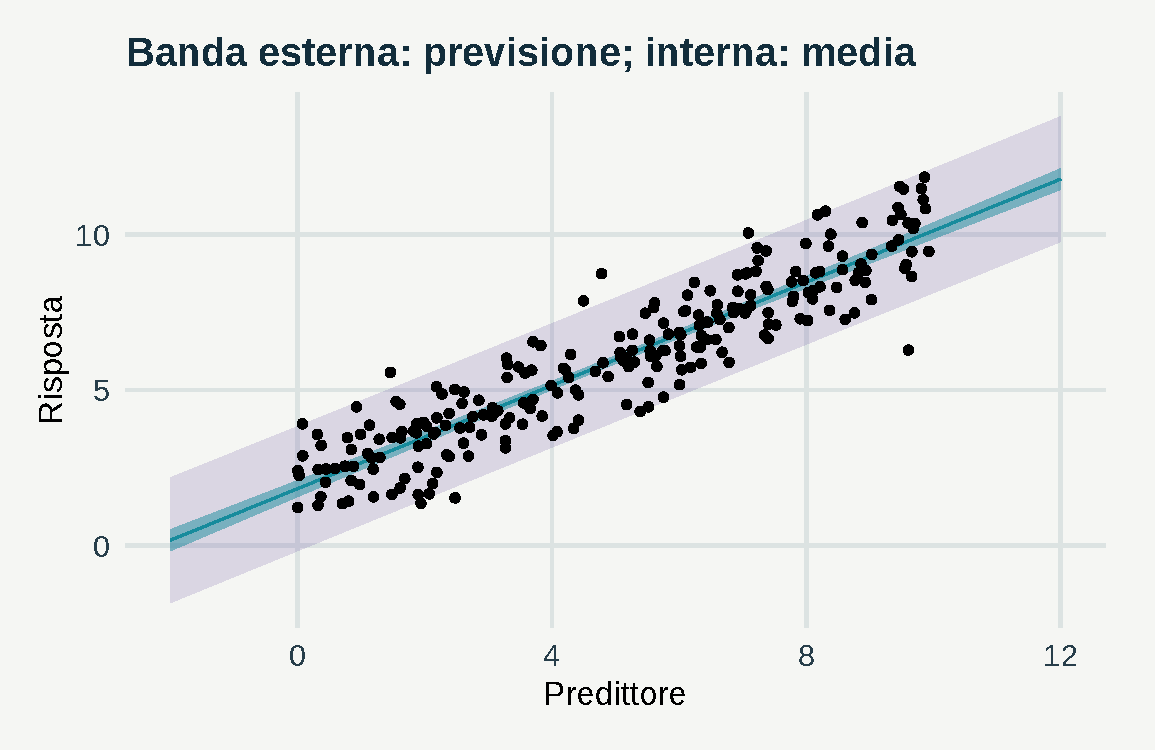
\includegraphics[width=\linewidth,height=5.6cm,keepaspectratio]{Esperimenti/m07-previsione-B.pdf}\par}
\PSmall{Numero di osservazioni: 60 $\to$ 240. Tutti gli altri parametri e il seme sono fissi.}
}};
\node[anchor=north west,inner sep=0] at([xshift=10.85cm,yshift=-2.12cm]current page.north west){\Colonna{8.16cm}{\PLabel{Confronto fra gli scenari}
{\fontsize{10.2}{12.8}\selectfont\begin{tabular}{@{}>{\raggedright\arraybackslash}p{0.48\linewidth}@{\hspace{.13cm}}>{\raggedright\arraybackslash}p{0.224\linewidth}@{\hspace{.13cm}}>{\raggedright\arraybackslash}p{0.224\linewidth}@{}}\toprule Grandezza & A & B\\[2.3pt]
\midrule 
SD residua & 1,2 & 1,01\\[2.3pt]
R² & 0,788 & 0,849\\[2.3pt]
\bottomrule\end{tabular}\par}
\vspace{.25cm}\PBody{Con 240 osservazioni la deviazione standard residua passa da 1,2 a 1,01 e R² da 0,788 a 0,849, due stime dello stesso rumore. La fascia della media si restringe con la numerosità, mentre quella per una nuova osservazione resta ampia almeno quanto la deviazione residua.}
}};
\node[anchor=north east,inner sep=0] at([xshift=17.1cm,yshift=-12.04cm]current page.north west){\fontsize{7.7}{9}\selectfont \href{https://marzione00.github.io/Lab_Geo/\#laboratorio/m07-previsione}{\color{Classical}\bfseries Apri il laboratorio · m07-previsione}};
\end{tikzpicture}\end{frame}

\begin{frame}[plain]\hypertarget{slide30}{}
\bookmark[level=1,page=30]{Dal risultato alla relazione}
\begin{tikzpicture}[remember picture,overlay]
\PilotChrome{Dal risultato alla relazione}{SINTESI}{30}{Distingui pendenza media, intervallo per un nuovo evento ed errore sugli eventi separati, con le rispettive unità.}
\node[anchor=north west,inner sep=0] at([xshift=.96cm,yshift=-2.12cm]current page.north west){\Colonna{9.40cm}{\PLabel{Domanda di partenza}
\PBody{Quanto migliora la previsione dell’attesa alla successiva eruzione se si conosce la durata di quella appena conclusa?}
\PLabel{Risultato da discutere}
\PBody{Nel campione di adattamento la pendenza è circa 10,90 minuti di attesa per minuto di durata, con intervallo HC3 da 10,19 a 11,61. Sugli 82 eventi di verifica l’errore quadratico medio scende da 12,77 minuti della previsione costante a 5,85 della retta, e l’intervallo di previsione copre 80 eventi.}
}};
\node[anchor=north west,inner sep=0] at([xshift=10.85cm,yshift=-2.12cm]current page.north west){\Colonna{8.16cm}{\PLabel{Limiti della conclusione}
\PBody{La durata è nota soltanto al termine dell’eruzione e l’estratto non documenta date e protocollo dei tempi. Entro i due addensamenti le pendenze valgono circa 5,59 e 4,33, per cui la retta globale riassume anche la separazione fra gruppi.}
\vspace{.4cm}\href{https://marzione00.github.io/Lab_Geo/\#modulo-P05}{\color{Classical}\bfseries Prosegui · P05 · CO$_2$: tendenza e calendario stagionale}
}};
\end{tikzpicture}\end{frame}

\begin{frame}[plain]\hypertarget{slide31}{}
\bookmark[level=1,page=31]{Fonti, dati e codice per riprodurre le figure}
\begin{tikzpicture}[remember picture,overlay]
\PilotChrome{Fonti, dati e codice per riprodurre le figure}{RIFERIMENTI}{31}{I risultati numerici si riferiscono ai dati e alle ipotesi dichiarate nel caso.}
\node[anchor=north west,inner sep=0] at([xshift=.96cm,yshift=-2.12cm]current page.north west){\Colonna{9.40cm}{\PLabel{Dati e attribuzioni}
\PBody{Dataset faithful del pacchetto datasets di R (Azzalini e Bowman, 1990): durate e attese del geyser Old Faithful, nel Parco di Yellowstone. La covarianza HC3 segue MacKinnon e White, confrontata con HC3\_se di statsmodels.}
}};
\node[anchor=north west,inner sep=0] at([xshift=10.85cm,yshift=-2.12cm]current page.north west){\Colonna{8.16cm}{\PLabel{Nell’archivio dei sorgenti}
\PBody{Codice contiene i frammenti delle pagine; R contiene lo script P04\_figure.R, che ricostruisce figure e valori dai dati. Esperimenti comprende i programmi dei due scenari, Diagrammi i disegni TikZ modificabili, Scena il modello Blender della copertina.}
\vspace{.4cm}\href{https://marzione00.github.io/Lab_Geo/\#modulo-P04}{\color{Classical}\bfseries Apri la spedizione P04 su GeoStat Lab}
}};
\end{tikzpicture}\end{frame}
\end{document}
